% Options for packages loaded elsewhere
\PassOptionsToPackage{unicode}{hyperref}
\PassOptionsToPackage{hyphens}{url}
%
\documentclass[
]{article}
\usepackage{lmodern}
\usepackage{amssymb,amsmath}
\usepackage{ifxetex,ifluatex}
\ifnum 0\ifxetex 1\fi\ifluatex 1\fi=0 % if pdftex
  \usepackage[T1]{fontenc}
  \usepackage[utf8]{inputenc}
  \usepackage{textcomp} % provide euro and other symbols
\else % if luatex or xetex
  \usepackage{unicode-math}
  \defaultfontfeatures{Scale=MatchLowercase}
  \defaultfontfeatures[\rmfamily]{Ligatures=TeX,Scale=1}
\fi
% Use upquote if available, for straight quotes in verbatim environments
\IfFileExists{upquote.sty}{\usepackage{upquote}}{}
\IfFileExists{microtype.sty}{% use microtype if available
  \usepackage[]{microtype}
  \UseMicrotypeSet[protrusion]{basicmath} % disable protrusion for tt fonts
}{}
\makeatletter
\@ifundefined{KOMAClassName}{% if non-KOMA class
  \IfFileExists{parskip.sty}{%
    \usepackage{parskip}
  }{% else
    \setlength{\parindent}{0pt}
    \setlength{\parskip}{6pt plus 2pt minus 1pt}}
}{% if KOMA class
  \KOMAoptions{parskip=half}}
\makeatother
\usepackage{xcolor}
\IfFileExists{xurl.sty}{\usepackage{xurl}}{} % add URL line breaks if available
\IfFileExists{bookmark.sty}{\usepackage{bookmark}}{\usepackage{hyperref}}
\hypersetup{
  pdftitle={RProjectST501\_PDF\_Part2},
  pdfauthor={Brock Akerman},
  hidelinks,
  pdfcreator={LaTeX via pandoc}}
\urlstyle{same} % disable monospaced font for URLs
\usepackage[margin=1in]{geometry}
\usepackage{color}
\usepackage{fancyvrb}
\newcommand{\VerbBar}{|}
\newcommand{\VERB}{\Verb[commandchars=\\\{\}]}
\DefineVerbatimEnvironment{Highlighting}{Verbatim}{commandchars=\\\{\}}
% Add ',fontsize=\small' for more characters per line
\usepackage{framed}
\definecolor{shadecolor}{RGB}{248,248,248}
\newenvironment{Shaded}{\begin{snugshade}}{\end{snugshade}}
\newcommand{\AlertTok}[1]{\textcolor[rgb]{0.94,0.16,0.16}{#1}}
\newcommand{\AnnotationTok}[1]{\textcolor[rgb]{0.56,0.35,0.01}{\textbf{\textit{#1}}}}
\newcommand{\AttributeTok}[1]{\textcolor[rgb]{0.77,0.63,0.00}{#1}}
\newcommand{\BaseNTok}[1]{\textcolor[rgb]{0.00,0.00,0.81}{#1}}
\newcommand{\BuiltInTok}[1]{#1}
\newcommand{\CharTok}[1]{\textcolor[rgb]{0.31,0.60,0.02}{#1}}
\newcommand{\CommentTok}[1]{\textcolor[rgb]{0.56,0.35,0.01}{\textit{#1}}}
\newcommand{\CommentVarTok}[1]{\textcolor[rgb]{0.56,0.35,0.01}{\textbf{\textit{#1}}}}
\newcommand{\ConstantTok}[1]{\textcolor[rgb]{0.00,0.00,0.00}{#1}}
\newcommand{\ControlFlowTok}[1]{\textcolor[rgb]{0.13,0.29,0.53}{\textbf{#1}}}
\newcommand{\DataTypeTok}[1]{\textcolor[rgb]{0.13,0.29,0.53}{#1}}
\newcommand{\DecValTok}[1]{\textcolor[rgb]{0.00,0.00,0.81}{#1}}
\newcommand{\DocumentationTok}[1]{\textcolor[rgb]{0.56,0.35,0.01}{\textbf{\textit{#1}}}}
\newcommand{\ErrorTok}[1]{\textcolor[rgb]{0.64,0.00,0.00}{\textbf{#1}}}
\newcommand{\ExtensionTok}[1]{#1}
\newcommand{\FloatTok}[1]{\textcolor[rgb]{0.00,0.00,0.81}{#1}}
\newcommand{\FunctionTok}[1]{\textcolor[rgb]{0.00,0.00,0.00}{#1}}
\newcommand{\ImportTok}[1]{#1}
\newcommand{\InformationTok}[1]{\textcolor[rgb]{0.56,0.35,0.01}{\textbf{\textit{#1}}}}
\newcommand{\KeywordTok}[1]{\textcolor[rgb]{0.13,0.29,0.53}{\textbf{#1}}}
\newcommand{\NormalTok}[1]{#1}
\newcommand{\OperatorTok}[1]{\textcolor[rgb]{0.81,0.36,0.00}{\textbf{#1}}}
\newcommand{\OtherTok}[1]{\textcolor[rgb]{0.56,0.35,0.01}{#1}}
\newcommand{\PreprocessorTok}[1]{\textcolor[rgb]{0.56,0.35,0.01}{\textit{#1}}}
\newcommand{\RegionMarkerTok}[1]{#1}
\newcommand{\SpecialCharTok}[1]{\textcolor[rgb]{0.00,0.00,0.00}{#1}}
\newcommand{\SpecialStringTok}[1]{\textcolor[rgb]{0.31,0.60,0.02}{#1}}
\newcommand{\StringTok}[1]{\textcolor[rgb]{0.31,0.60,0.02}{#1}}
\newcommand{\VariableTok}[1]{\textcolor[rgb]{0.00,0.00,0.00}{#1}}
\newcommand{\VerbatimStringTok}[1]{\textcolor[rgb]{0.31,0.60,0.02}{#1}}
\newcommand{\WarningTok}[1]{\textcolor[rgb]{0.56,0.35,0.01}{\textbf{\textit{#1}}}}
\usepackage{graphicx,grffile}
\makeatletter
\def\maxwidth{\ifdim\Gin@nat@width>\linewidth\linewidth\else\Gin@nat@width\fi}
\def\maxheight{\ifdim\Gin@nat@height>\textheight\textheight\else\Gin@nat@height\fi}
\makeatother
% Scale images if necessary, so that they will not overflow the page
% margins by default, and it is still possible to overwrite the defaults
% using explicit options in \includegraphics[width, height, ...]{}
\setkeys{Gin}{width=\maxwidth,height=\maxheight,keepaspectratio}
% Set default figure placement to htbp
\makeatletter
\def\fps@figure{htbp}
\makeatother
\setlength{\emergencystretch}{3em} % prevent overfull lines
\providecommand{\tightlist}{%
  \setlength{\itemsep}{0pt}\setlength{\parskip}{0pt}}
\setcounter{secnumdepth}{-\maxdimen} % remove section numbering

\title{RProjectST501\_PDF\_Part2}
\author{Brock Akerman}
\date{11/16/2020}

\begin{document}
\maketitle

\begin{verbatim}
## Warning: package 'tidyverse' was built under R version 4.0.2
\end{verbatim}

\begin{verbatim}
## -- Attaching packages ---------------------------------------------------------------------------------------- tidyverse 1.3.0 --
\end{verbatim}

\begin{verbatim}
## v ggplot2 3.3.0     v purrr   0.3.4
## v tibble  3.0.1     v dplyr   0.8.5
## v tidyr   1.0.2     v stringr 1.4.0
## v readr   1.3.1     v forcats 0.5.0
\end{verbatim}

\begin{verbatim}
## -- Conflicts ------------------------------------------------------------------------------------------- tidyverse_conflicts() --
## x dplyr::filter() masks stats::filter()
## x dplyr::lag()    masks stats::lag()
\end{verbatim}

\begin{verbatim}
## Warning: package 'rmarkdown' was built under R version 4.0.3
\end{verbatim}

\begin{verbatim}
## Warning: package 'viridis' was built under R version 4.0.3
\end{verbatim}

\begin{verbatim}
## Loading required package: viridisLite
\end{verbatim}

Part 2: ``Visualizing Convergence in Distribution'' This part will
consider how well the Central Limit Theorem applies to sample means from
Poisson data

Consider a sample size of n = 5 from a Poisson distribution with rate
parameter λ = 1. Generate N = 50000 data sets of size n from the Poisson
distribution.

\begin{Shaded}
\begin{Highlighting}[]
\NormalTok{m =}\StringTok{ }\DecValTok{5}
\NormalTok{lambda =}\StringTok{ }\DecValTok{1}
\NormalTok{M =}\StringTok{ }\DecValTok{50000}
\NormalTok{ds2 <-}\StringTok{ }\KeywordTok{matrix}\NormalTok{(}\KeywordTok{replicate}\NormalTok{(M,(}\KeywordTok{rpois}\NormalTok{(m,}\DecValTok{1}\NormalTok{))),}\DataTypeTok{nrow=}\DecValTok{50000}\NormalTok{,}\DataTypeTok{ncol=}\DecValTok{5}\NormalTok{)}
\end{Highlighting}
\end{Shaded}

For each data set, find the sample mean value. Hint If you saved the
above data in a large matrix the colMeans or rowMeans functions can be
handy here), e.g., n \textless- 5 N \textless- 50000 A matrix of N =
50000 rows, each rows containing n = 5 sample from a Poisson
distribution with rate 1 X \textless- matrix(rpois(n*N, λ = 1), nrow =
N), rowMeans(X) \#\# This will give you a vector of N = 50000 sample
means.

\begin{Shaded}
\begin{Highlighting}[]
\NormalTok{rMeans <-}\StringTok{ }\KeywordTok{matrix}\NormalTok{(}\KeywordTok{rowMeans}\NormalTok{(ds2),}\DataTypeTok{nrow=}\DecValTok{50000}\NormalTok{,}\DataTypeTok{ncol=}\DecValTok{1}\NormalTok{);}
\end{Highlighting}
\end{Shaded}

Create a histogram of the sample means. Make the bins of appropriate
width so that each bin only has one value of the support. For instance,
the possible values for the sample mean here are 0, 0.2, 0.4, 0.6, . .
.. Make sure that each bar only has one of these values included (so the
bins would go from say −0.1 to 0.1, 0.1 to 0.3, 0.3 to 0.5. The use of
the breaks argument for the histogram function hist will be helpful
here. The central limit theorem says that ¯X \textasciitilde{} N(λ, λ/n)
when ¯X is the sample mean of n i.i.d Pois(λ) random variables. Overlay
this large-sample distribution on the histogram (Hint:use freq = FALSE
in your histogram and the curve function with add = TRUE to overlay the
normal distribution). All plots should have appropriate titles and axis
labels.

\begin{Shaded}
\begin{Highlighting}[]
\KeywordTok{par}\NormalTok{(}\DataTypeTok{bg=}\StringTok{"gray"}\NormalTok{)}
\NormalTok{binlen <-}\StringTok{ }\KeywordTok{c}\NormalTok{(}\OperatorTok{-}\FloatTok{0.1}\NormalTok{,}\FloatTok{0.1}\NormalTok{,}\FloatTok{0.3}\NormalTok{,}\FloatTok{0.5}\NormalTok{,}\FloatTok{0.7}\NormalTok{,}\FloatTok{0.9}\NormalTok{,}\FloatTok{1.1}\NormalTok{,}\FloatTok{1.3}\NormalTok{,}\FloatTok{1.5}\NormalTok{,}\FloatTok{1.7}\NormalTok{,}\FloatTok{1.9}\NormalTok{,}\FloatTok{2.1}\NormalTok{,}\FloatTok{2.3}\NormalTok{,}\FloatTok{2.5}\NormalTok{,}\FloatTok{2.7}\NormalTok{,}\FloatTok{2.9}\NormalTok{,}\FloatTok{3.1}\NormalTok{,}\FloatTok{3.3}\NormalTok{,}\FloatTok{3.5}\NormalTok{,}\FloatTok{3.7}\NormalTok{,}\FloatTok{3.9}\NormalTok{,}\FloatTok{4.1}\NormalTok{);}
\KeywordTok{hist}\NormalTok{(rMeans ,}\DataTypeTok{breaks=}\NormalTok{binlen ,}\DataTypeTok{main=}\StringTok{"Visualizing Convergence in Distribution"}\NormalTok{ ,}\DataTypeTok{xlab=}\StringTok{"sample poisson means"}\NormalTok{ ,}\DataTypeTok{xlim=}\KeywordTok{c}\NormalTok{(}\OperatorTok{-}\FloatTok{0.5}\NormalTok{,}\FloatTok{2.5}\NormalTok{) ,}\DataTypeTok{ylab=}\StringTok{"density"}\NormalTok{ ,}\DataTypeTok{ylim=}\KeywordTok{c}\NormalTok{(}\DecValTok{0}\NormalTok{,}\FloatTok{1.1}\NormalTok{) ,}\DataTypeTok{freq =} \OtherTok{FALSE}\NormalTok{)}
\NormalTok{x <-}\StringTok{ }\KeywordTok{seq}\NormalTok{(}\OperatorTok{-}\DecValTok{4}\NormalTok{,}\DecValTok{5}\NormalTok{, }\DataTypeTok{by =} \FloatTok{0.1}\NormalTok{)}
\NormalTok{y <-}\StringTok{ }\KeywordTok{dnorm}\NormalTok{(x, }\DataTypeTok{mean =}\NormalTok{ lambda, }\DataTypeTok{sd =}\NormalTok{ lambda}\OperatorTok{/}\KeywordTok{sqrt}\NormalTok{(m))}
\KeywordTok{curve}\NormalTok{(}\KeywordTok{dnorm}\NormalTok{(x, }\DataTypeTok{mean=}\NormalTok{lambda, }\DataTypeTok{sd=}\NormalTok{lambda}\OperatorTok{/}\KeywordTok{sqrt}\NormalTok{(m)), }\DataTypeTok{add=}\OtherTok{TRUE}\NormalTok{, }\DataTypeTok{col=}\StringTok{"orange"}\NormalTok{, }\DataTypeTok{lwd=}\DecValTok{2}\NormalTok{)}
\end{Highlighting}
\end{Shaded}

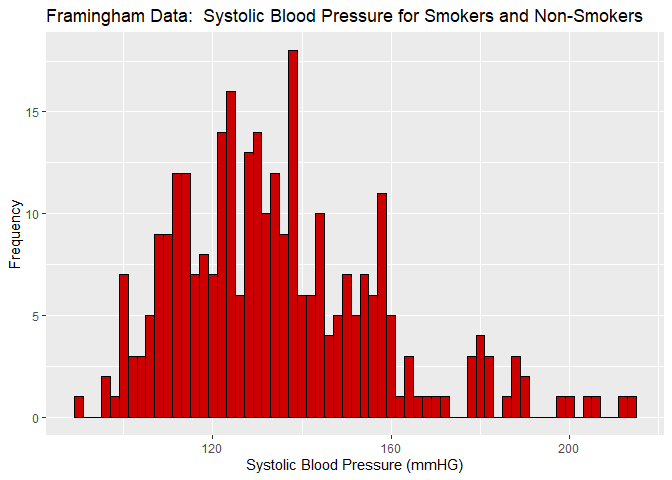
\includegraphics{RProjectST501_BrockAkerman_Part2_files/figure-latex/unnamed-chunk-4-1.pdf}

Use the N = 50000 {[}mean{]} values to approximate the probability that
¯X is greater than or equal to λ + 2λ/sqrt(n). Also report this
probability as approximated by the normal distribution.

\begin{Shaded}
\begin{Highlighting}[]
\NormalTok{TF_values}\FloatTok{.2}\NormalTok{ <-}\StringTok{ }\NormalTok{rMeans }\OperatorTok{>=}\StringTok{ }\NormalTok{(lambda}\OperatorTok{+}\NormalTok{((}\DecValTok{2}\OperatorTok{*}\NormalTok{lambda)}\OperatorTok{/}\KeywordTok{sqrt}\NormalTok{(m)))}
\NormalTok{TFprob <-}\StringTok{ }\KeywordTok{sum}\NormalTok{(TF_values}\FloatTok{.2}\NormalTok{)}\OperatorTok{/}\NormalTok{M}
\KeywordTok{print}\NormalTok{(}\DecValTok{1}\OperatorTok{-}\NormalTok{TFprob)}
\end{Highlighting}
\end{Shaded}

\begin{verbatim}
## [1] 0.9693
\end{verbatim}

\begin{Shaded}
\begin{Highlighting}[]
\NormalTok{NormProb <-}\StringTok{ }\DecValTok{1}\OperatorTok{-}\KeywordTok{dnorm}\NormalTok{((lambda}\OperatorTok{+}\NormalTok{((}\DecValTok{2}\OperatorTok{*}\NormalTok{lambda)}\OperatorTok{/}\KeywordTok{sqrt}\NormalTok{(m))),}\DataTypeTok{mean=}\NormalTok{lambda,}\DataTypeTok{sd=}\NormalTok{(lambda}\OperatorTok{/}\KeywordTok{sqrt}\NormalTok{(m)))}
\KeywordTok{print}\NormalTok{(NormProb)}
\end{Highlighting}
\end{Shaded}

\begin{verbatim}
## [1] 0.8792725
\end{verbatim}

Repeat the above for n = 10, n = 30, and n = 100. FOR m = 1,λ = 1

\begin{Shaded}
\begin{Highlighting}[]
\NormalTok{m1 =}\StringTok{ }\DecValTok{1}\NormalTok{; lambda}\FloatTok{.1}\NormalTok{ =}\StringTok{ }\DecValTok{1}\NormalTok{; M =}\StringTok{ }\DecValTok{50000}
\NormalTok{ds1 <-}\StringTok{ }\KeywordTok{matrix}\NormalTok{(}\KeywordTok{replicate}\NormalTok{(M,(}\KeywordTok{rpois}\NormalTok{(m1,lambda}\FloatTok{.1}\NormalTok{))),}\DataTypeTok{nrow=}\DecValTok{50000}\NormalTok{,}\DataTypeTok{ncol=}\DecValTok{5}\NormalTok{)}
\NormalTok{rMeans1 <-}\StringTok{ }\KeywordTok{matrix}\NormalTok{(}\KeywordTok{rowMeans}\NormalTok{(ds1),}\DataTypeTok{nrow=}\DecValTok{50000}\NormalTok{,}\DataTypeTok{ncol=}\DecValTok{1}\NormalTok{)}
\NormalTok{binlen <-}\StringTok{ }\KeywordTok{c}\NormalTok{(}\OperatorTok{-}\FloatTok{0.5}\NormalTok{,}\FloatTok{0.5}\NormalTok{,}\FloatTok{1.5}\NormalTok{,}\FloatTok{2.5}\NormalTok{,}\FloatTok{3.5}\NormalTok{,}\FloatTok{4.5}\NormalTok{,}\FloatTok{5.5}\NormalTok{,}\FloatTok{6.5}\NormalTok{,}\FloatTok{7.5}\NormalTok{,}\FloatTok{8.5}\NormalTok{,}\FloatTok{9.5}\NormalTok{,}\FloatTok{10.5}\NormalTok{,}\FloatTok{11.5}\NormalTok{,}\FloatTok{12.5}\NormalTok{,}\FloatTok{13.5}\NormalTok{,}\FloatTok{14.5}\NormalTok{,}\FloatTok{15.5}\NormalTok{,}\FloatTok{16.5}\NormalTok{,}\FloatTok{17.5}\NormalTok{,}\FloatTok{18.5}\NormalTok{,}\FloatTok{19.5}\NormalTok{,}\FloatTok{20.5}\NormalTok{,}\FloatTok{21.5}\NormalTok{,}\FloatTok{22.5}\NormalTok{);}
\KeywordTok{hist}\NormalTok{(rMeans1,}\DataTypeTok{breaks=}\NormalTok{binlen ,}\DataTypeTok{main=}\StringTok{"Pois(λ) and Normal(λ,λ/m) curve of 50,000 replicated means where m=1,λ=1"}\NormalTok{ ,}\DataTypeTok{xlab=}\StringTok{"sample poisson means"}\NormalTok{ ,}\DataTypeTok{xlim=}\KeywordTok{c}\NormalTok{(}\DecValTok{0}\NormalTok{,}\DecValTok{5}\NormalTok{) ,}\DataTypeTok{ylab=}\StringTok{"density"}\NormalTok{ ,}\DataTypeTok{ylim=}\KeywordTok{c}\NormalTok{(}\DecValTok{0}\NormalTok{,}\DecValTok{1}\NormalTok{) ,}\DataTypeTok{freq =} \OtherTok{FALSE}\NormalTok{, }\DataTypeTok{col=}\KeywordTok{viridis}\NormalTok{(}\DecValTok{4}\NormalTok{))}
\NormalTok{x <-}\StringTok{ }\KeywordTok{seq}\NormalTok{(}\DecValTok{0}\NormalTok{,}\DecValTok{2}\NormalTok{, }\DataTypeTok{by =} \FloatTok{0.2}\NormalTok{)}
\NormalTok{y1 <-}\StringTok{ }\KeywordTok{dnorm}\NormalTok{(x, }\DataTypeTok{mean=}\NormalTok{lambda}\FloatTok{.1}\NormalTok{, }\DataTypeTok{sd=}\NormalTok{lambda}\FloatTok{.1}\OperatorTok{/}\NormalTok{(}\KeywordTok{sqrt}\NormalTok{(m1)))}
\KeywordTok{curve}\NormalTok{(}\KeywordTok{dnorm}\NormalTok{(x, }\DataTypeTok{mean=}\NormalTok{lambda}\FloatTok{.1}\NormalTok{, }\DataTypeTok{sd=}\NormalTok{(lambda}\FloatTok{.1}\OperatorTok{/}\KeywordTok{sqrt}\NormalTok{(m1))), }\DataTypeTok{add=}\OtherTok{TRUE}\NormalTok{, }\DataTypeTok{col=}\StringTok{"#cc0000"}\NormalTok{, }\DataTypeTok{lwd=}\DecValTok{2}\NormalTok{)}
\end{Highlighting}
\end{Shaded}

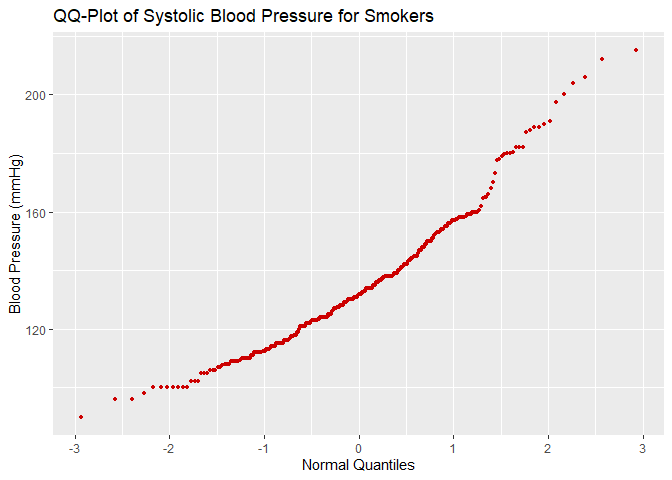
\includegraphics{RProjectST501_BrockAkerman_Part2_files/figure-latex/unnamed-chunk-6-1.pdf}

\begin{Shaded}
\begin{Highlighting}[]
\NormalTok{TF_values}\FloatTok{.1}\NormalTok{ <-}\StringTok{ }\NormalTok{rMeans1 }\OperatorTok{>=}\StringTok{ }\NormalTok{(lambda}\FloatTok{.1}\OperatorTok{+}\NormalTok{((}\DecValTok{2}\OperatorTok{*}\NormalTok{lambda}\FloatTok{.1}\NormalTok{)}\OperatorTok{/}\KeywordTok{sqrt}\NormalTok{(m1)))}
\NormalTok{TFprob1 <-}\StringTok{ }\KeywordTok{sum}\NormalTok{(TF_values}\FloatTok{.1}\NormalTok{)}\OperatorTok{/}\NormalTok{M; }\KeywordTok{print}\NormalTok{(TFprob1)}
\end{Highlighting}
\end{Shaded}

\begin{verbatim}
## [1] 0.07974
\end{verbatim}

\begin{Shaded}
\begin{Highlighting}[]
\NormalTok{NormProb1 <-}\StringTok{ }\KeywordTok{dnorm}\NormalTok{((lambda}\FloatTok{.1}\OperatorTok{+}\NormalTok{((}\DecValTok{2}\OperatorTok{*}\NormalTok{lambda}\FloatTok{.1}\NormalTok{)}\OperatorTok{/}\KeywordTok{sqrt}\NormalTok{(m1))),}\DataTypeTok{mean=}\NormalTok{lambda}\FloatTok{.1}\NormalTok{,}\DataTypeTok{sd=}\NormalTok{(lambda}\FloatTok{.1}\OperatorTok{/}\KeywordTok{sqrt}\NormalTok{(m1))); }\KeywordTok{print}\NormalTok{(NormProb1)}
\end{Highlighting}
\end{Shaded}

\begin{verbatim}
## [1] 0.05399097
\end{verbatim}

FOR m = 10,λ = 1

\begin{Shaded}
\begin{Highlighting}[]
\NormalTok{m10 =}\StringTok{ }\DecValTok{10}\NormalTok{; lambda}\FloatTok{.1}\NormalTok{ =}\StringTok{ }\DecValTok{1}\NormalTok{; M =}\StringTok{ }\DecValTok{50000}
\NormalTok{ds10 <-}\StringTok{ }\KeywordTok{matrix}\NormalTok{(}\KeywordTok{replicate}\NormalTok{(M,(}\KeywordTok{rpois}\NormalTok{(m10,}\DecValTok{1}\NormalTok{))),}\DataTypeTok{nrow=}\DecValTok{50000}\NormalTok{,}\DataTypeTok{ncol=}\DecValTok{5}\NormalTok{)}
\NormalTok{rMeans10 <-}\StringTok{ }\KeywordTok{matrix}\NormalTok{(}\KeywordTok{rowMeans}\NormalTok{(ds10),}\DataTypeTok{nrow=}\DecValTok{50000}\NormalTok{,}\DataTypeTok{ncol=}\DecValTok{1}\NormalTok{)}
\NormalTok{binlen <-}\StringTok{ }\KeywordTok{c}\NormalTok{(}\OperatorTok{-}\FloatTok{5.1}\NormalTok{,}\OperatorTok{-}\FloatTok{4.9}\NormalTok{,}\OperatorTok{-}\FloatTok{4.7}\NormalTok{,}\OperatorTok{-}\FloatTok{4.5}\NormalTok{,}\OperatorTok{-}\FloatTok{4.3}\NormalTok{,}\OperatorTok{-}\FloatTok{4.1}\NormalTok{,}\OperatorTok{-}\FloatTok{3.9}\NormalTok{,}\OperatorTok{-}\FloatTok{3.7}\NormalTok{,}\OperatorTok{-}\FloatTok{3.5}\NormalTok{,}\OperatorTok{-}\FloatTok{3.3}\NormalTok{,}\OperatorTok{-}\FloatTok{3.1}\NormalTok{,}\OperatorTok{-}\FloatTok{2.9}\NormalTok{,}\OperatorTok{-}\FloatTok{2.7}\NormalTok{,}\OperatorTok{-}\FloatTok{2.5}\NormalTok{,}\OperatorTok{-}\FloatTok{2.3}\NormalTok{,}\OperatorTok{-}\FloatTok{2.1}\NormalTok{,}\OperatorTok{-}\FloatTok{1.9}\NormalTok{,}\OperatorTok{-}\FloatTok{1.7}\NormalTok{,}\OperatorTok{-}\FloatTok{1.5}\NormalTok{,}\OperatorTok{-}\FloatTok{1.3}\NormalTok{,}\OperatorTok{-}\FloatTok{1.1}\NormalTok{,}\OperatorTok{-}\FloatTok{0.9}\NormalTok{,}\OperatorTok{-}\FloatTok{0.7}\NormalTok{,}\OperatorTok{-}\FloatTok{0.5}\NormalTok{,}\OperatorTok{-}\FloatTok{0.3}\NormalTok{,}\OperatorTok{-}\FloatTok{0.1}\NormalTok{,}\FloatTok{0.1}\NormalTok{,}\FloatTok{0.3}\NormalTok{,}\FloatTok{0.5}\NormalTok{,}\FloatTok{0.7}\NormalTok{,}\FloatTok{0.9}\NormalTok{,}\FloatTok{1.1}\NormalTok{,}\FloatTok{1.3}\NormalTok{,}\FloatTok{1.5}\NormalTok{,}\FloatTok{1.7}\NormalTok{,}\FloatTok{1.9}\NormalTok{,}\FloatTok{2.1}\NormalTok{,}\FloatTok{2.3}\NormalTok{,}\FloatTok{2.5}\NormalTok{,}\FloatTok{2.7}\NormalTok{,}\FloatTok{2.9}\NormalTok{,}\FloatTok{3.1}\NormalTok{,}\FloatTok{3.3}\NormalTok{,}\FloatTok{3.5}\NormalTok{,}\FloatTok{3.7}\NormalTok{,}\FloatTok{3.9}\NormalTok{,}\FloatTok{4.1}\NormalTok{,}\FloatTok{4.3}\NormalTok{,}\FloatTok{4.5}\NormalTok{,}\FloatTok{4.7}\NormalTok{,}\FloatTok{4.9}\NormalTok{,}\FloatTok{5.1}\NormalTok{)}
\KeywordTok{hist}\NormalTok{(rMeans10,}\DataTypeTok{breaks=}\NormalTok{binlen ,}\DataTypeTok{main=}\StringTok{"Pois(λ) and Normal(λ,λ/m) curve of 50,000 replicated means where m=10,λ=1"}\NormalTok{ ,}\DataTypeTok{xlab=}\StringTok{"sample poisson means"}\NormalTok{ ,}\DataTypeTok{xlim=}\KeywordTok{c}\NormalTok{(}\OperatorTok{-}\FloatTok{0.1}\NormalTok{,}\FloatTok{2.5}\NormalTok{) ,}\DataTypeTok{ylab=}\StringTok{"density"}\NormalTok{ ,}\DataTypeTok{ylim=}\KeywordTok{c}\NormalTok{(}\DecValTok{0}\NormalTok{,}\DecValTok{4}\NormalTok{) ,}\DataTypeTok{freq =} \OtherTok{FALSE}\NormalTok{, }\DataTypeTok{col=}\KeywordTok{viridis}\NormalTok{(}\DecValTok{19}\NormalTok{))}
\NormalTok{x <-}\StringTok{ }\KeywordTok{seq}\NormalTok{(}\DecValTok{0}\NormalTok{,}\DecValTok{2}\NormalTok{, }\DataTypeTok{by =} \FloatTok{0.2}\NormalTok{)}
\NormalTok{y10 <-}\StringTok{ }\KeywordTok{dnorm}\NormalTok{(x, }\DataTypeTok{mean=}\NormalTok{lambda}\FloatTok{.1}\NormalTok{, }\DataTypeTok{sd=}\NormalTok{lambda}\FloatTok{.1}\OperatorTok{/}\NormalTok{(}\KeywordTok{sqrt}\NormalTok{(m10)))}
\KeywordTok{curve}\NormalTok{(}\KeywordTok{dnorm}\NormalTok{(x, }\DataTypeTok{mean=}\NormalTok{lambda}\FloatTok{.1}\NormalTok{, }\DataTypeTok{sd=}\NormalTok{(lambda}\FloatTok{.1}\OperatorTok{/}\KeywordTok{sqrt}\NormalTok{(m10))), }\DataTypeTok{add=}\OtherTok{TRUE}\NormalTok{, }\DataTypeTok{col=}\StringTok{"#cc0000"}\NormalTok{, }\DataTypeTok{lwd=}\DecValTok{2}\NormalTok{)}
\end{Highlighting}
\end{Shaded}

\includegraphics{RProjectST501_BrockAkerman_Part2_files/figure-latex/unnamed-chunk-7-1.pdf}

\begin{Shaded}
\begin{Highlighting}[]
\NormalTok{TF_values}\FloatTok{.10}\NormalTok{ <-}\StringTok{ }\NormalTok{rMeans10 }\OperatorTok{>=}\StringTok{ }\NormalTok{(lambda}\FloatTok{.1}\OperatorTok{+}\NormalTok{((}\DecValTok{2}\OperatorTok{*}\NormalTok{lambda}\FloatTok{.1}\NormalTok{)}\OperatorTok{/}\KeywordTok{sqrt}\NormalTok{(m10)))}
\NormalTok{TFprob10 <-}\StringTok{ }\KeywordTok{sum}\NormalTok{(TF_values}\FloatTok{.10}\NormalTok{)}\OperatorTok{/}\NormalTok{M; }\KeywordTok{print}\NormalTok{(TFprob10)}
\end{Highlighting}
\end{Shaded}

\begin{verbatim}
## [1] 0.0686
\end{verbatim}

\begin{Shaded}
\begin{Highlighting}[]
\NormalTok{NormProb10 <-}\StringTok{ }\KeywordTok{dnorm}\NormalTok{((lambda}\FloatTok{.1}\OperatorTok{+}\NormalTok{((}\DecValTok{2}\OperatorTok{*}\NormalTok{lambda}\FloatTok{.1}\NormalTok{)}\OperatorTok{/}\KeywordTok{sqrt}\NormalTok{(m10))),}\DataTypeTok{mean=}\NormalTok{lambda}\FloatTok{.1}\NormalTok{,}\DataTypeTok{sd=}\NormalTok{(lambda}\FloatTok{.1}\OperatorTok{/}\KeywordTok{sqrt}\NormalTok{(m10))); }\KeywordTok{print}\NormalTok{(NormProb10)}
\end{Highlighting}
\end{Shaded}

\begin{verbatim}
## [1] 0.1707344
\end{verbatim}

FOR m = 30,λ = 1

\begin{Shaded}
\begin{Highlighting}[]
\NormalTok{m30 =}\StringTok{ }\DecValTok{30}\NormalTok{; lambda}\FloatTok{.1}\NormalTok{ =}\StringTok{ }\DecValTok{1}\NormalTok{; M =}\StringTok{ }\DecValTok{30000}
\NormalTok{ds30 <-}\StringTok{ }\KeywordTok{matrix}\NormalTok{(}\KeywordTok{replicate}\NormalTok{(M,(}\KeywordTok{rpois}\NormalTok{(m30,}\DecValTok{1}\NormalTok{))),}\DataTypeTok{nrow=}\DecValTok{30000}\NormalTok{,}\DataTypeTok{ncol=}\DecValTok{5}\NormalTok{)}
\NormalTok{rMeans30 <-}\StringTok{ }\KeywordTok{matrix}\NormalTok{(}\KeywordTok{rowMeans}\NormalTok{(ds30),}\DataTypeTok{nrow=}\DecValTok{30000}\NormalTok{,}\DataTypeTok{ncol=}\DecValTok{1}\NormalTok{)}
\NormalTok{binlen <-}\StringTok{ }\KeywordTok{c}\NormalTok{(}\OperatorTok{-}\FloatTok{5.1}\NormalTok{,}\OperatorTok{-}\FloatTok{4.9}\NormalTok{,}\OperatorTok{-}\FloatTok{4.7}\NormalTok{,}\OperatorTok{-}\FloatTok{4.5}\NormalTok{,}\OperatorTok{-}\FloatTok{4.3}\NormalTok{,}\OperatorTok{-}\FloatTok{4.1}\NormalTok{,}\OperatorTok{-}\FloatTok{3.9}\NormalTok{,}\OperatorTok{-}\FloatTok{3.7}\NormalTok{,}\OperatorTok{-}\FloatTok{3.5}\NormalTok{,}\OperatorTok{-}\FloatTok{3.3}\NormalTok{,}\OperatorTok{-}\FloatTok{3.1}\NormalTok{,}\OperatorTok{-}\FloatTok{2.9}\NormalTok{,}\OperatorTok{-}\FloatTok{2.7}\NormalTok{,}\OperatorTok{-}\FloatTok{2.5}\NormalTok{,}\OperatorTok{-}\FloatTok{2.3}\NormalTok{,}\OperatorTok{-}\FloatTok{2.1}\NormalTok{,}\OperatorTok{-}\FloatTok{1.9}\NormalTok{,}\OperatorTok{-}\FloatTok{1.7}\NormalTok{,}\OperatorTok{-}\FloatTok{1.5}\NormalTok{,}\OperatorTok{-}\FloatTok{1.3}\NormalTok{,}\OperatorTok{-}\FloatTok{1.1}\NormalTok{,}\OperatorTok{-}\FloatTok{0.9}\NormalTok{,}\OperatorTok{-}\FloatTok{0.7}\NormalTok{,}\OperatorTok{-}\FloatTok{0.5}\NormalTok{,}\OperatorTok{-}\FloatTok{0.3}\NormalTok{,}\OperatorTok{-}\FloatTok{0.1}\NormalTok{,}\FloatTok{0.1}\NormalTok{,}\FloatTok{0.3}\NormalTok{,}\FloatTok{0.5}\NormalTok{,}\FloatTok{0.7}\NormalTok{,}\FloatTok{0.9}\NormalTok{,}\FloatTok{1.1}\NormalTok{,}\FloatTok{1.3}\NormalTok{,}\FloatTok{1.5}\NormalTok{,}\FloatTok{1.7}\NormalTok{,}\FloatTok{1.9}\NormalTok{,}\FloatTok{2.1}\NormalTok{,}\FloatTok{2.3}\NormalTok{,}\FloatTok{2.5}\NormalTok{,}\FloatTok{2.7}\NormalTok{,}\FloatTok{2.9}\NormalTok{,}\FloatTok{3.1}\NormalTok{,}\FloatTok{3.3}\NormalTok{,}\FloatTok{3.5}\NormalTok{,}\FloatTok{3.7}\NormalTok{,}\FloatTok{3.9}\NormalTok{,}\FloatTok{4.1}\NormalTok{,}\FloatTok{4.3}\NormalTok{,}\FloatTok{4.5}\NormalTok{,}\FloatTok{4.7}\NormalTok{,}\FloatTok{4.9}\NormalTok{,}\FloatTok{5.1}\NormalTok{)}
\KeywordTok{hist}\NormalTok{(rMeans30,}\DataTypeTok{breaks=}\NormalTok{binlen ,}\DataTypeTok{main=}\StringTok{"Pois(λ) and Normal(λ,λ/m) curve of 50,000 replicated means where m=30,λ=1"}\NormalTok{ ,}\DataTypeTok{xlab=}\StringTok{"sample poisson means"}\NormalTok{ ,}\DataTypeTok{xlim=}\KeywordTok{c}\NormalTok{(}\OperatorTok{-}\FloatTok{0.1}\NormalTok{,}\FloatTok{2.5}\NormalTok{) ,}\DataTypeTok{ylab=}\StringTok{"density"}\NormalTok{ ,}\DataTypeTok{ylim=}\KeywordTok{c}\NormalTok{(}\DecValTok{0}\NormalTok{,}\DecValTok{4}\NormalTok{) ,}\DataTypeTok{freq =} \OtherTok{FALSE}\NormalTok{, }\DataTypeTok{col=}\KeywordTok{viridis}\NormalTok{(}\DecValTok{19}\NormalTok{))}
\NormalTok{x <-}\StringTok{ }\KeywordTok{seq}\NormalTok{(}\DecValTok{0}\NormalTok{,}\DecValTok{2}\NormalTok{, }\DataTypeTok{by =} \FloatTok{0.2}\NormalTok{)}
\NormalTok{y30 <-}\StringTok{ }\KeywordTok{dnorm}\NormalTok{(x, }\DataTypeTok{mean=}\NormalTok{lambda}\FloatTok{.1}\NormalTok{, }\DataTypeTok{sd=}\NormalTok{lambda}\FloatTok{.1}\OperatorTok{/}\NormalTok{(}\KeywordTok{sqrt}\NormalTok{(m30)))}
\KeywordTok{curve}\NormalTok{(}\KeywordTok{dnorm}\NormalTok{(x, }\DataTypeTok{mean=}\NormalTok{lambda}\FloatTok{.1}\NormalTok{, }\DataTypeTok{sd=}\NormalTok{(lambda}\FloatTok{.1}\OperatorTok{/}\KeywordTok{sqrt}\NormalTok{(m30))), }\DataTypeTok{add=}\OtherTok{TRUE}\NormalTok{, }\DataTypeTok{col=}\StringTok{"#FF0033"}\NormalTok{, }\DataTypeTok{lwd=}\DecValTok{2}\NormalTok{)}
\end{Highlighting}
\end{Shaded}

\includegraphics{RProjectST501_BrockAkerman_Part2_files/figure-latex/unnamed-chunk-8-1.pdf}

\begin{Shaded}
\begin{Highlighting}[]
\NormalTok{TF_values}\FloatTok{.30}\NormalTok{ <-}\StringTok{ }\NormalTok{rMeans30 }\OperatorTok{>=}\StringTok{ }\NormalTok{(lambda}\FloatTok{.1}\OperatorTok{+}\NormalTok{((}\DecValTok{2}\OperatorTok{*}\NormalTok{lambda}\FloatTok{.1}\NormalTok{)}\OperatorTok{/}\KeywordTok{sqrt}\NormalTok{(m30)))}
\NormalTok{TFprob30 <-}\StringTok{ }\KeywordTok{sum}\NormalTok{(TF_values}\FloatTok{.30}\NormalTok{)}\OperatorTok{/}\NormalTok{M; }\KeywordTok{print}\NormalTok{(TFprob30)}
\end{Highlighting}
\end{Shaded}

\begin{verbatim}
## [1] 0.2392667
\end{verbatim}

\begin{Shaded}
\begin{Highlighting}[]
\NormalTok{NormProb30 <-}\StringTok{ }\KeywordTok{dnorm}\NormalTok{((lambda}\FloatTok{.1}\OperatorTok{+}\NormalTok{((}\DecValTok{2}\OperatorTok{*}\NormalTok{lambda}\FloatTok{.1}\NormalTok{)}\OperatorTok{/}\KeywordTok{sqrt}\NormalTok{(m30))),}\DataTypeTok{mean=}\NormalTok{lambda}\FloatTok{.1}\NormalTok{,}\DataTypeTok{sd=}\NormalTok{(lambda}\FloatTok{.1}\OperatorTok{/}\KeywordTok{sqrt}\NormalTok{(m30))); }\KeywordTok{print}\NormalTok{(NormProb30)}
\end{Highlighting}
\end{Shaded}

\begin{verbatim}
## [1] 0.2957207
\end{verbatim}

FOR m = 100,λ = 1

\begin{Shaded}
\begin{Highlighting}[]
\NormalTok{m100 =}\StringTok{ }\DecValTok{100}\NormalTok{; lambda}\FloatTok{.1}\NormalTok{ =}\StringTok{ }\DecValTok{1}\NormalTok{; M =}\StringTok{ }\DecValTok{50000}
\NormalTok{ds100 <-}\StringTok{ }\KeywordTok{matrix}\NormalTok{(}\KeywordTok{replicate}\NormalTok{(M,(}\KeywordTok{rpois}\NormalTok{(m100,}\DecValTok{1}\NormalTok{))),}\DataTypeTok{nrow=}\DecValTok{50000}\NormalTok{,}\DataTypeTok{ncol=}\DecValTok{5}\NormalTok{)}
\NormalTok{rMeans100 <-}\StringTok{ }\KeywordTok{matrix}\NormalTok{(}\KeywordTok{rowMeans}\NormalTok{(ds100),}\DataTypeTok{nrow=}\DecValTok{50000}\NormalTok{,}\DataTypeTok{ncol=}\DecValTok{1}\NormalTok{)}
\NormalTok{binlen <-}\StringTok{ }\KeywordTok{c}\NormalTok{(}\OperatorTok{-}\FloatTok{5.1}\NormalTok{,}\OperatorTok{-}\FloatTok{4.9}\NormalTok{,}\OperatorTok{-}\FloatTok{4.7}\NormalTok{,}\OperatorTok{-}\FloatTok{4.5}\NormalTok{,}\OperatorTok{-}\FloatTok{4.3}\NormalTok{,}\OperatorTok{-}\FloatTok{4.1}\NormalTok{,}\OperatorTok{-}\FloatTok{3.9}\NormalTok{,}\OperatorTok{-}\FloatTok{3.7}\NormalTok{,}\OperatorTok{-}\FloatTok{3.5}\NormalTok{,}\OperatorTok{-}\FloatTok{3.3}\NormalTok{,}\OperatorTok{-}\FloatTok{3.1}\NormalTok{,}\OperatorTok{-}\FloatTok{2.9}\NormalTok{,}\OperatorTok{-}\FloatTok{2.7}\NormalTok{,}\OperatorTok{-}\FloatTok{2.5}\NormalTok{,}\OperatorTok{-}\FloatTok{2.3}\NormalTok{,}\OperatorTok{-}\FloatTok{2.1}\NormalTok{,}\OperatorTok{-}\FloatTok{1.9}\NormalTok{,}\OperatorTok{-}\FloatTok{1.7}\NormalTok{,}\OperatorTok{-}\FloatTok{1.5}\NormalTok{,}\OperatorTok{-}\FloatTok{1.3}\NormalTok{,}\OperatorTok{-}\FloatTok{1.1}\NormalTok{,}\OperatorTok{-}\FloatTok{0.9}\NormalTok{,}\OperatorTok{-}\FloatTok{0.7}\NormalTok{,}\OperatorTok{-}\FloatTok{0.5}\NormalTok{,}\OperatorTok{-}\FloatTok{0.3}\NormalTok{,}\OperatorTok{-}\FloatTok{0.1}\NormalTok{,}\FloatTok{0.1}\NormalTok{,}\FloatTok{0.3}\NormalTok{,}\FloatTok{0.5}\NormalTok{,}\FloatTok{0.7}\NormalTok{,}\FloatTok{0.9}\NormalTok{,}\FloatTok{1.1}\NormalTok{,}\FloatTok{1.3}\NormalTok{,}\FloatTok{1.5}\NormalTok{,}\FloatTok{1.7}\NormalTok{,}\FloatTok{1.9}\NormalTok{,}\FloatTok{2.1}\NormalTok{,}\FloatTok{2.3}\NormalTok{,}\FloatTok{2.5}\NormalTok{,}\FloatTok{2.7}\NormalTok{,}\FloatTok{2.9}\NormalTok{,}\FloatTok{3.1}\NormalTok{,}\FloatTok{3.3}\NormalTok{,}\FloatTok{3.5}\NormalTok{,}\FloatTok{3.7}\NormalTok{,}\FloatTok{3.9}\NormalTok{,}\FloatTok{4.1}\NormalTok{,}\FloatTok{4.3}\NormalTok{,}\FloatTok{4.5}\NormalTok{,}\FloatTok{4.7}\NormalTok{,}\FloatTok{4.9}\NormalTok{,}\FloatTok{5.1}\NormalTok{)}
\KeywordTok{hist}\NormalTok{(rMeans100,}\DataTypeTok{breaks=}\NormalTok{binlen ,}\DataTypeTok{main=}\StringTok{"Pois(λ) and Normal(λ,λ/m) curve of 50,000 replicated means where m=100,λ=1"}\NormalTok{ ,}\DataTypeTok{xlab=}\StringTok{"sample poisson means"}\NormalTok{ ,}\DataTypeTok{xlim=}\KeywordTok{c}\NormalTok{(}\OperatorTok{-}\FloatTok{0.1}\NormalTok{,}\FloatTok{2.5}\NormalTok{) ,}\DataTypeTok{ylab=}\StringTok{"density"}\NormalTok{ ,}\DataTypeTok{ylim=}\KeywordTok{c}\NormalTok{(}\DecValTok{0}\NormalTok{,}\DecValTok{4}\NormalTok{) ,}\DataTypeTok{freq =} \OtherTok{FALSE}\NormalTok{, }\DataTypeTok{col=}\KeywordTok{viridis}\NormalTok{(}\DecValTok{19}\NormalTok{))}
\NormalTok{x <-}\StringTok{ }\KeywordTok{seq}\NormalTok{(}\DecValTok{0}\NormalTok{,}\DecValTok{2}\NormalTok{, }\DataTypeTok{by =} \FloatTok{0.2}\NormalTok{)}
\NormalTok{y100 <-}\StringTok{ }\KeywordTok{dnorm}\NormalTok{(x, }\DataTypeTok{mean=}\NormalTok{lambda}\FloatTok{.1}\NormalTok{, }\DataTypeTok{sd=}\NormalTok{lambda}\FloatTok{.1}\OperatorTok{/}\NormalTok{(}\KeywordTok{sqrt}\NormalTok{(m100)))}
\KeywordTok{curve}\NormalTok{(}\KeywordTok{dnorm}\NormalTok{(x, }\DataTypeTok{mean=}\NormalTok{lambda}\FloatTok{.1}\NormalTok{, }\DataTypeTok{sd=}\NormalTok{(lambda}\FloatTok{.1}\OperatorTok{/}\KeywordTok{sqrt}\NormalTok{(m100))), }\DataTypeTok{add=}\OtherTok{TRUE}\NormalTok{, }\DataTypeTok{col=}\StringTok{"#FF0033"}\NormalTok{, }\DataTypeTok{lwd=}\DecValTok{2}\NormalTok{)}
\end{Highlighting}
\end{Shaded}

\includegraphics{RProjectST501_BrockAkerman_Part2_files/figure-latex/unnamed-chunk-9-1.pdf}

\begin{Shaded}
\begin{Highlighting}[]
\NormalTok{TF_values}\FloatTok{.100}\NormalTok{ <-}\StringTok{ }\NormalTok{rMeans100 }\OperatorTok{>=}\StringTok{ }\NormalTok{(lambda}\FloatTok{.1}\OperatorTok{+}\NormalTok{((}\DecValTok{2}\OperatorTok{*}\NormalTok{lambda}\FloatTok{.1}\NormalTok{)}\OperatorTok{/}\KeywordTok{sqrt}\NormalTok{(m100)))}
\NormalTok{TFprob100 <-}\StringTok{ }\KeywordTok{sum}\NormalTok{(TF_values}\FloatTok{.100}\NormalTok{)}\OperatorTok{/}\NormalTok{M; }\KeywordTok{print}\NormalTok{(TFprob100)}
\end{Highlighting}
\end{Shaded}

\begin{verbatim}
## [1] 0.38572
\end{verbatim}

\begin{Shaded}
\begin{Highlighting}[]
\NormalTok{NormProb100 <-}\StringTok{ }\KeywordTok{dnorm}\NormalTok{((lambda}\FloatTok{.1}\OperatorTok{+}\NormalTok{((}\DecValTok{2}\OperatorTok{*}\NormalTok{lambda}\FloatTok{.1}\NormalTok{)}\OperatorTok{/}\KeywordTok{sqrt}\NormalTok{(m100))),}\DataTypeTok{mean=}\NormalTok{lambda}\FloatTok{.1}\NormalTok{,}\DataTypeTok{sd=}\NormalTok{(lambda}\FloatTok{.1}\OperatorTok{/}\KeywordTok{sqrt}\NormalTok{(m100))); }\KeywordTok{print}\NormalTok{(NormProb100)}
\end{Highlighting}
\end{Shaded}

\begin{verbatim}
## [1] 0.5399097
\end{verbatim}

Repeat all of the above for λ = 5 and λ = 25. You should have a total of
12 scenarios/plots FOR m = 1,λ = 5

\begin{Shaded}
\begin{Highlighting}[]
\NormalTok{m1 =}\StringTok{ }\DecValTok{1}\NormalTok{; lambda}\FloatTok{.5}\NormalTok{ =}\StringTok{ }\DecValTok{5}\NormalTok{; M =}\StringTok{ }\DecValTok{50000}
\NormalTok{ds1 <-}\StringTok{ }\KeywordTok{matrix}\NormalTok{(}\KeywordTok{replicate}\NormalTok{(M,(}\KeywordTok{rpois}\NormalTok{(m1,lambda}\FloatTok{.5}\NormalTok{))),}\DataTypeTok{nrow=}\DecValTok{50000}\NormalTok{,}\DataTypeTok{ncol=}\DecValTok{5}\NormalTok{)}
\NormalTok{rMeans1 <-}\StringTok{ }\KeywordTok{matrix}\NormalTok{(}\KeywordTok{rowMeans}\NormalTok{(ds1),}\DataTypeTok{nrow=}\DecValTok{50000}\NormalTok{,}\DataTypeTok{ncol=}\DecValTok{1}\NormalTok{)}
\NormalTok{binlen <-}\StringTok{ }\KeywordTok{c}\NormalTok{(}\OperatorTok{-}\FloatTok{0.5}\NormalTok{,}\FloatTok{0.5}\NormalTok{,}\FloatTok{1.5}\NormalTok{,}\FloatTok{2.5}\NormalTok{,}\FloatTok{3.5}\NormalTok{,}\FloatTok{4.5}\NormalTok{,}\FloatTok{5.5}\NormalTok{,}\FloatTok{6.5}\NormalTok{,}\FloatTok{7.5}\NormalTok{,}\FloatTok{8.5}\NormalTok{,}\FloatTok{9.5}\NormalTok{,}\FloatTok{10.5}\NormalTok{,}\FloatTok{11.5}\NormalTok{,}\FloatTok{12.5}\NormalTok{,}\FloatTok{13.5}\NormalTok{,}\FloatTok{14.5}\NormalTok{,}\FloatTok{15.5}\NormalTok{,}\FloatTok{16.5}\NormalTok{,}\FloatTok{17.5}\NormalTok{,}\FloatTok{18.5}\NormalTok{,}\FloatTok{19.5}\NormalTok{,}\FloatTok{20.5}\NormalTok{,}\FloatTok{21.5}\NormalTok{,}\FloatTok{22.5}\NormalTok{,}\FloatTok{23.5}\NormalTok{,}\FloatTok{24.5}\NormalTok{,}\FloatTok{25.5}\NormalTok{,}\FloatTok{26.5}\NormalTok{,}\FloatTok{27.5}\NormalTok{,}\FloatTok{28.5}\NormalTok{,}\FloatTok{29.5}\NormalTok{,}\FloatTok{30.5}\NormalTok{)}
\KeywordTok{hist}\NormalTok{(rMeans1,}\DataTypeTok{breaks=}\NormalTok{binlen ,}\DataTypeTok{main=}\StringTok{"Pois(λ) and Normal(λ,λ/m) curve of 50,000 replicated means where m=1,λ=5"}\NormalTok{ ,}\DataTypeTok{xlab=}\StringTok{"sample poisson means"}\NormalTok{ ,}\DataTypeTok{xlim=}\KeywordTok{c}\NormalTok{(}\DecValTok{0}\NormalTok{,}\DecValTok{16}\NormalTok{) ,}\DataTypeTok{ylab=}\StringTok{"density"}\NormalTok{ ,}\DataTypeTok{ylim=}\KeywordTok{c}\NormalTok{(}\DecValTok{0}\NormalTok{,}\FloatTok{0.3}\NormalTok{) ,}\DataTypeTok{freq =} \OtherTok{FALSE}\NormalTok{, }\DataTypeTok{col=}\KeywordTok{magma}\NormalTok{(}\DecValTok{13}\NormalTok{))}
\NormalTok{x <-}\StringTok{ }\KeywordTok{seq}\NormalTok{(}\OperatorTok{-}\DecValTok{4}\NormalTok{,}\DecValTok{5}\NormalTok{, }\DataTypeTok{by =} \FloatTok{0.1}\NormalTok{)}
\NormalTok{y1 <-}\StringTok{ }\KeywordTok{dnorm}\NormalTok{(x, }\DataTypeTok{mean =}\NormalTok{ lambda}\FloatTok{.5}\NormalTok{, }\DataTypeTok{sd =}\NormalTok{ lambda}\FloatTok{.5}\OperatorTok{/}\KeywordTok{sqrt}\NormalTok{(m1))}
\KeywordTok{curve}\NormalTok{(}\KeywordTok{dnorm}\NormalTok{(x, }\DataTypeTok{mean=}\NormalTok{lambda}\FloatTok{.5}\NormalTok{, }\DataTypeTok{sd=}\NormalTok{lambda}\FloatTok{.5}\OperatorTok{/}\KeywordTok{sqrt}\NormalTok{(m1)), }\DataTypeTok{add=}\OtherTok{TRUE}\NormalTok{, }\DataTypeTok{col=}\StringTok{"#66CC00"}\NormalTok{, }\DataTypeTok{lwd=}\DecValTok{2}\NormalTok{)}
\end{Highlighting}
\end{Shaded}

\includegraphics{RProjectST501_BrockAkerman_Part2_files/figure-latex/unnamed-chunk-10-1.pdf}

\begin{Shaded}
\begin{Highlighting}[]
\NormalTok{TF_values}\FloatTok{.1}\NormalTok{ <-}\StringTok{ }\NormalTok{rMeans1 }\OperatorTok{>=}\StringTok{ }\NormalTok{(lambda}\FloatTok{.5}\OperatorTok{+}\NormalTok{((}\DecValTok{2}\OperatorTok{*}\NormalTok{lambda}\FloatTok{.5}\NormalTok{)}\OperatorTok{/}\KeywordTok{sqrt}\NormalTok{(m1)))}
\NormalTok{TFprob1 <-}\StringTok{ }\KeywordTok{sum}\NormalTok{(TF_values}\FloatTok{.1}\NormalTok{)}\OperatorTok{/}\NormalTok{M; }\KeywordTok{print}\NormalTok{(TFprob1)}
\end{Highlighting}
\end{Shaded}

\begin{verbatim}
## [1] 2e-04
\end{verbatim}

\begin{Shaded}
\begin{Highlighting}[]
\NormalTok{NormProb1 <-}\StringTok{ }\KeywordTok{dnorm}\NormalTok{((lambda}\FloatTok{.5}\OperatorTok{+}\NormalTok{((}\DecValTok{2}\OperatorTok{*}\NormalTok{lambda}\FloatTok{.5}\NormalTok{)}\OperatorTok{/}\KeywordTok{sqrt}\NormalTok{(m1))),}\DataTypeTok{mean=}\NormalTok{lambda}\FloatTok{.5}\NormalTok{,}\DataTypeTok{sd=}\NormalTok{(lambda}\FloatTok{.5}\OperatorTok{/}\KeywordTok{sqrt}\NormalTok{(m1))); }\KeywordTok{print}\NormalTok{(NormProb1)}
\end{Highlighting}
\end{Shaded}

\begin{verbatim}
## [1] 0.01079819
\end{verbatim}

FOR m = 10,λ = 5

\begin{Shaded}
\begin{Highlighting}[]
\NormalTok{m10 =}\StringTok{ }\DecValTok{10}\NormalTok{; lambda}\FloatTok{.5}\NormalTok{ =}\StringTok{ }\DecValTok{5}\NormalTok{; M =}\StringTok{ }\DecValTok{50000}
\NormalTok{ds10 <-}\StringTok{ }\KeywordTok{matrix}\NormalTok{(}\KeywordTok{replicate}\NormalTok{(M,(}\KeywordTok{rpois}\NormalTok{(m10,lambda}\FloatTok{.5}\NormalTok{))),}\DataTypeTok{nrow=}\DecValTok{50000}\NormalTok{,}\DataTypeTok{ncol=}\DecValTok{5}\NormalTok{)}
\NormalTok{rMeans10 <-}\StringTok{ }\KeywordTok{matrix}\NormalTok{(}\KeywordTok{rowMeans}\NormalTok{(ds10),}\DataTypeTok{nrow=}\DecValTok{50000}\NormalTok{,}\DataTypeTok{ncol=}\DecValTok{1}\NormalTok{)}
\NormalTok{binlen <-}\StringTok{ }\KeywordTok{c}\NormalTok{(}\OperatorTok{-}\FloatTok{0.1}\NormalTok{,}\FloatTok{0.1}\NormalTok{,}\FloatTok{0.3}\NormalTok{,}\FloatTok{0.5}\NormalTok{,}\FloatTok{0.7}\NormalTok{,}\FloatTok{0.9}\NormalTok{,}\FloatTok{1.1}\NormalTok{,}\FloatTok{1.3}\NormalTok{,}\FloatTok{1.5}\NormalTok{,}\FloatTok{1.7}\NormalTok{,}\FloatTok{1.9}\NormalTok{,}\FloatTok{2.1}\NormalTok{,}\FloatTok{2.3}\NormalTok{,}\FloatTok{2.5}\NormalTok{,}\FloatTok{2.7}\NormalTok{,}\FloatTok{2.9}\NormalTok{,}\FloatTok{3.1}\NormalTok{,}\FloatTok{3.3}\NormalTok{,}\FloatTok{3.5}\NormalTok{,}\FloatTok{3.7}\NormalTok{,}\FloatTok{3.9}\NormalTok{,}\FloatTok{4.1}\NormalTok{,}\FloatTok{4.3}\NormalTok{,}\FloatTok{4.5}\NormalTok{,}\FloatTok{4.7}\NormalTok{,}\FloatTok{4.9}\NormalTok{,}\FloatTok{5.1}\NormalTok{,}\FloatTok{5.3}\NormalTok{,}\FloatTok{5.5}\NormalTok{,}\FloatTok{5.7}\NormalTok{,}\FloatTok{5.9}\NormalTok{,}\FloatTok{6.1}\NormalTok{,}\FloatTok{6.3}\NormalTok{,}\FloatTok{6.5}\NormalTok{,}\FloatTok{6.7}\NormalTok{,}\FloatTok{6.9}\NormalTok{,}\FloatTok{7.1}\NormalTok{,}\FloatTok{7.3}\NormalTok{,}\FloatTok{7.5}\NormalTok{,}\FloatTok{7.7}\NormalTok{,}\FloatTok{7.9}\NormalTok{,}\FloatTok{8.1}\NormalTok{,}\FloatTok{8.3}\NormalTok{,}\FloatTok{8.5}\NormalTok{,}\FloatTok{8.7}\NormalTok{,}\FloatTok{8.9}\NormalTok{,}\FloatTok{9.1}\NormalTok{,}\FloatTok{9.3}\NormalTok{,}\FloatTok{9.5}\NormalTok{,}\FloatTok{9.7}\NormalTok{,}\FloatTok{9.9}\NormalTok{,}\FloatTok{10.1}\NormalTok{,}\FloatTok{10.3}\NormalTok{,}\FloatTok{10.5}\NormalTok{,}\FloatTok{10.7}\NormalTok{,}\FloatTok{10.9}\NormalTok{,}\FloatTok{11.1}\NormalTok{,}\FloatTok{11.3}\NormalTok{,}\FloatTok{11.5}\NormalTok{,}\FloatTok{11.7}\NormalTok{,}\FloatTok{11.9}\NormalTok{)}
\KeywordTok{hist}\NormalTok{(rMeans10,}\DataTypeTok{breaks=}\NormalTok{binlen ,}\DataTypeTok{main=}\StringTok{"Pois(λ) and Normal(λ,λ/m) curve of 50,000 replicated means where m=10,λ=5"}\NormalTok{ ,}\DataTypeTok{xlab=}\StringTok{"sample poisson means"}\NormalTok{ ,}\DataTypeTok{xlim=}\KeywordTok{c}\NormalTok{(}\DecValTok{2}\NormalTok{,}\FloatTok{8.5}\NormalTok{) ,}\DataTypeTok{ylab=}\StringTok{"density"}\NormalTok{ ,}\DataTypeTok{ylim=}\KeywordTok{c}\NormalTok{(}\DecValTok{0}\NormalTok{,}\FloatTok{1.1}\NormalTok{) ,}\DataTypeTok{freq =} \OtherTok{FALSE}\NormalTok{, }\DataTypeTok{col=}\KeywordTok{magma}\NormalTok{(}\DecValTok{50}\NormalTok{))}
\NormalTok{x <-}\StringTok{ }\KeywordTok{seq}\NormalTok{(}\OperatorTok{-}\DecValTok{4}\NormalTok{,}\DecValTok{5}\NormalTok{, }\DataTypeTok{by =} \FloatTok{0.1}\NormalTok{)}
\NormalTok{y10 <-}\StringTok{ }\KeywordTok{dnorm}\NormalTok{(x, }\DataTypeTok{mean =}\NormalTok{ lambda}\FloatTok{.5}\NormalTok{, }\DataTypeTok{sd =}\NormalTok{ lambda}\FloatTok{.5}\OperatorTok{/}\KeywordTok{sqrt}\NormalTok{(m10))}
\KeywordTok{curve}\NormalTok{(}\KeywordTok{dnorm}\NormalTok{(x, }\DataTypeTok{mean=}\NormalTok{lambda}\FloatTok{.5}\NormalTok{, }\DataTypeTok{sd=}\NormalTok{lambda}\FloatTok{.5}\OperatorTok{/}\KeywordTok{sqrt}\NormalTok{(m10)), }\DataTypeTok{add=}\OtherTok{TRUE}\NormalTok{, }\DataTypeTok{col=}\StringTok{"#66CC00"}\NormalTok{, }\DataTypeTok{lwd=}\DecValTok{2}\NormalTok{)}
\end{Highlighting}
\end{Shaded}

\includegraphics{RProjectST501_BrockAkerman_Part2_files/figure-latex/unnamed-chunk-11-1.pdf}

\begin{Shaded}
\begin{Highlighting}[]
\NormalTok{TF_values}\FloatTok{.10}\NormalTok{ <-}\StringTok{ }\NormalTok{rMeans10 }\OperatorTok{>=}\StringTok{ }\NormalTok{(lambda}\FloatTok{.5}\OperatorTok{+}\NormalTok{((}\DecValTok{2}\OperatorTok{*}\NormalTok{lambda}\FloatTok{.5}\NormalTok{)}\OperatorTok{/}\KeywordTok{sqrt}\NormalTok{(m10)))}
\NormalTok{TFprob10 <-}\StringTok{ }\KeywordTok{sum}\NormalTok{(TF_values}\FloatTok{.10}\NormalTok{)}\OperatorTok{/}\NormalTok{M; }\KeywordTok{print}\NormalTok{(TFprob10)}
\end{Highlighting}
\end{Shaded}

\begin{verbatim}
## [1] 0.00162
\end{verbatim}

\begin{Shaded}
\begin{Highlighting}[]
\NormalTok{NormProb10 <-}\StringTok{ }\KeywordTok{dnorm}\NormalTok{((lambda}\FloatTok{.5}\OperatorTok{+}\NormalTok{((}\DecValTok{2}\OperatorTok{*}\NormalTok{lambda}\FloatTok{.5}\NormalTok{)}\OperatorTok{/}\KeywordTok{sqrt}\NormalTok{(m10))),}\DataTypeTok{mean=}\NormalTok{lambda}\FloatTok{.5}\NormalTok{,}\DataTypeTok{sd=}\NormalTok{(lambda}\FloatTok{.5}\OperatorTok{/}\KeywordTok{sqrt}\NormalTok{(m10))); }\KeywordTok{print}\NormalTok{(NormProb10)}
\end{Highlighting}
\end{Shaded}

\begin{verbatim}
## [1] 0.03414689
\end{verbatim}

FOR m = 30,λ = 5

\begin{Shaded}
\begin{Highlighting}[]
\NormalTok{m30 =}\StringTok{ }\DecValTok{30}\NormalTok{; lambda}\FloatTok{.5}\NormalTok{ =}\StringTok{ }\DecValTok{5}\NormalTok{; M =}\StringTok{ }\DecValTok{30000}
\NormalTok{ds30 <-}\StringTok{ }\KeywordTok{matrix}\NormalTok{(}\KeywordTok{replicate}\NormalTok{(M,(}\KeywordTok{rpois}\NormalTok{(m30,lambda}\FloatTok{.5}\NormalTok{))),}\DataTypeTok{nrow=}\DecValTok{30000}\NormalTok{,}\DataTypeTok{ncol=}\DecValTok{5}\NormalTok{)}
\NormalTok{rMeans30 <-}\StringTok{ }\KeywordTok{matrix}\NormalTok{(}\KeywordTok{rowMeans}\NormalTok{(ds30),}\DataTypeTok{nrow=}\DecValTok{30000}\NormalTok{,}\DataTypeTok{ncol=}\DecValTok{1}\NormalTok{)}
\NormalTok{binlen <-}\StringTok{ }\KeywordTok{c}\NormalTok{(}\OperatorTok{-}\FloatTok{0.1}\NormalTok{,}\FloatTok{0.1}\NormalTok{,}\FloatTok{0.3}\NormalTok{,}\FloatTok{0.5}\NormalTok{,}\FloatTok{0.7}\NormalTok{,}\FloatTok{0.9}\NormalTok{,}\FloatTok{1.1}\NormalTok{,}\FloatTok{1.3}\NormalTok{,}\FloatTok{1.5}\NormalTok{,}\FloatTok{1.7}\NormalTok{,}\FloatTok{1.9}\NormalTok{,}\FloatTok{2.1}\NormalTok{,}\FloatTok{2.3}\NormalTok{,}\FloatTok{2.5}\NormalTok{,}\FloatTok{2.7}\NormalTok{,}\FloatTok{2.9}\NormalTok{,}\FloatTok{3.1}\NormalTok{,}\FloatTok{3.3}\NormalTok{,}\FloatTok{3.5}\NormalTok{,}\FloatTok{3.7}\NormalTok{,}\FloatTok{3.9}\NormalTok{,}\FloatTok{4.1}\NormalTok{,}\FloatTok{4.3}\NormalTok{,}\FloatTok{4.5}\NormalTok{,}\FloatTok{4.7}\NormalTok{,}\FloatTok{4.9}\NormalTok{,}\FloatTok{5.1}\NormalTok{,}\FloatTok{5.3}\NormalTok{,}\FloatTok{5.5}\NormalTok{,}\FloatTok{5.7}\NormalTok{,}\FloatTok{5.9}\NormalTok{,}\FloatTok{6.1}\NormalTok{,}\FloatTok{6.3}\NormalTok{,}\FloatTok{6.5}\NormalTok{,}\FloatTok{6.7}\NormalTok{,}\FloatTok{6.9}\NormalTok{,}\FloatTok{7.1}\NormalTok{,}\FloatTok{7.3}\NormalTok{,}\FloatTok{7.5}\NormalTok{,}\FloatTok{7.7}\NormalTok{,}\FloatTok{7.9}\NormalTok{,}\FloatTok{8.1}\NormalTok{,}\FloatTok{8.3}\NormalTok{,}\FloatTok{8.5}\NormalTok{,}\FloatTok{8.7}\NormalTok{,}\FloatTok{8.9}\NormalTok{,}\FloatTok{9.1}\NormalTok{,}\FloatTok{9.3}\NormalTok{,}\FloatTok{9.5}\NormalTok{,}\FloatTok{9.7}\NormalTok{,}\FloatTok{9.9}\NormalTok{,}\FloatTok{10.1}\NormalTok{,}\FloatTok{10.3}\NormalTok{,}\FloatTok{10.5}\NormalTok{,}\FloatTok{10.7}\NormalTok{,}\FloatTok{10.9}\NormalTok{,}\FloatTok{11.1}\NormalTok{,}\FloatTok{11.3}\NormalTok{,}\FloatTok{11.5}\NormalTok{,}\FloatTok{11.7}\NormalTok{,}\FloatTok{11.9}\NormalTok{)}
\KeywordTok{hist}\NormalTok{(rMeans30,}\DataTypeTok{breaks=}\NormalTok{binlen ,}\DataTypeTok{main=}\StringTok{"Pois(λ) and Normal(λ,λ/m) curve of 50,000 replicated means where m=30,λ=5"}\NormalTok{ ,}\DataTypeTok{xlab=}\StringTok{"sample poisson means"}\NormalTok{ ,}\DataTypeTok{xlim=}\KeywordTok{c}\NormalTok{(}\DecValTok{2}\NormalTok{,}\FloatTok{8.5}\NormalTok{) ,}\DataTypeTok{ylab=}\StringTok{"density"}\NormalTok{ ,}\DataTypeTok{ylim=}\KeywordTok{c}\NormalTok{(}\DecValTok{0}\NormalTok{,}\FloatTok{1.1}\NormalTok{) ,}\DataTypeTok{freq =} \OtherTok{FALSE}\NormalTok{, }\DataTypeTok{col=}\KeywordTok{magma}\NormalTok{(}\DecValTok{50}\NormalTok{))}
\NormalTok{x30 <-}\StringTok{ }\KeywordTok{seq}\NormalTok{(}\OperatorTok{-}\DecValTok{4}\NormalTok{,}\DecValTok{5}\NormalTok{, }\DataTypeTok{by =} \FloatTok{0.1}\NormalTok{)}
\NormalTok{y30 <-}\StringTok{ }\KeywordTok{dnorm}\NormalTok{(x30, }\DataTypeTok{mean =}\NormalTok{ lambda}\FloatTok{.5}\NormalTok{, }\DataTypeTok{sd =}\NormalTok{ lambda}\FloatTok{.5}\OperatorTok{/}\KeywordTok{sqrt}\NormalTok{(m30))}
\KeywordTok{curve}\NormalTok{(}\KeywordTok{dnorm}\NormalTok{(x, }\DataTypeTok{mean=}\NormalTok{lambda}\FloatTok{.5}\NormalTok{, }\DataTypeTok{sd=}\NormalTok{lambda}\FloatTok{.5}\OperatorTok{/}\KeywordTok{sqrt}\NormalTok{(m30)), }\DataTypeTok{add=}\OtherTok{TRUE}\NormalTok{, }\DataTypeTok{col=}\StringTok{"#66CC00"}\NormalTok{, }\DataTypeTok{lwd=}\DecValTok{2}\NormalTok{)}
\end{Highlighting}
\end{Shaded}

\includegraphics{RProjectST501_BrockAkerman_Part2_files/figure-latex/unnamed-chunk-12-1.pdf}

\begin{Shaded}
\begin{Highlighting}[]
\NormalTok{TF_values}\FloatTok{.30}\NormalTok{ <-}\StringTok{ }\NormalTok{rMeans30 }\OperatorTok{>=}\StringTok{ }\NormalTok{(lambda}\FloatTok{.5}\OperatorTok{+}\NormalTok{((}\DecValTok{2}\OperatorTok{*}\NormalTok{lambda}\FloatTok{.5}\NormalTok{)}\OperatorTok{/}\KeywordTok{sqrt}\NormalTok{(m30)))}
\NormalTok{TFprob30 <-}\StringTok{ }\KeywordTok{sum}\NormalTok{(TF_values}\FloatTok{.30}\NormalTok{)}\OperatorTok{/}\NormalTok{M;}\KeywordTok{print}\NormalTok{(TFprob30)}
\end{Highlighting}
\end{Shaded}

\begin{verbatim}
## [1] 0.03316667
\end{verbatim}

\begin{Shaded}
\begin{Highlighting}[]
\NormalTok{NormProb30 <-}\StringTok{ }\KeywordTok{dnorm}\NormalTok{((lambda}\FloatTok{.5}\OperatorTok{+}\NormalTok{((}\DecValTok{2}\OperatorTok{*}\NormalTok{lambda}\FloatTok{.5}\NormalTok{)}\OperatorTok{/}\KeywordTok{sqrt}\NormalTok{(m30))),}\DataTypeTok{mean=}\NormalTok{lambda}\FloatTok{.5}\NormalTok{,}\DataTypeTok{sd=}\NormalTok{(lambda}\FloatTok{.5}\OperatorTok{/}\KeywordTok{sqrt}\NormalTok{(m30)));}\KeywordTok{print}\NormalTok{(NormProb30)}
\end{Highlighting}
\end{Shaded}

\begin{verbatim}
## [1] 0.05914414
\end{verbatim}

FOR m = 100,λ = 5

\begin{Shaded}
\begin{Highlighting}[]
\NormalTok{m100 =}\StringTok{ }\DecValTok{100}\NormalTok{; lambda}\FloatTok{.5}\NormalTok{ =}\StringTok{ }\DecValTok{5}\NormalTok{; M =}\StringTok{ }\DecValTok{50000}
\NormalTok{ds100 <-}\StringTok{ }\KeywordTok{matrix}\NormalTok{(}\KeywordTok{replicate}\NormalTok{(M,(}\KeywordTok{rpois}\NormalTok{(m100,lambda}\FloatTok{.5}\NormalTok{))),}\DataTypeTok{nrow=}\DecValTok{50000}\NormalTok{,}\DataTypeTok{ncol=}\DecValTok{5}\NormalTok{)}
\NormalTok{rMeans100 <-}\StringTok{ }\KeywordTok{matrix}\NormalTok{(}\KeywordTok{rowMeans}\NormalTok{(ds100),}\DataTypeTok{nrow=}\DecValTok{50000}\NormalTok{,}\DataTypeTok{ncol=}\DecValTok{1}\NormalTok{)}
\NormalTok{binlen <-}\StringTok{ }\KeywordTok{c}\NormalTok{(}\OperatorTok{-}\FloatTok{0.1}\NormalTok{,}\FloatTok{0.1}\NormalTok{,}\FloatTok{0.3}\NormalTok{,}\FloatTok{0.5}\NormalTok{,}\FloatTok{0.7}\NormalTok{,}\FloatTok{0.9}\NormalTok{,}\FloatTok{1.1}\NormalTok{,}\FloatTok{1.3}\NormalTok{,}\FloatTok{1.5}\NormalTok{,}\FloatTok{1.7}\NormalTok{,}\FloatTok{1.9}\NormalTok{,}\FloatTok{2.1}\NormalTok{,}\FloatTok{2.3}\NormalTok{,}\FloatTok{2.5}\NormalTok{,}\FloatTok{2.7}\NormalTok{,}\FloatTok{2.9}\NormalTok{,}\FloatTok{3.1}\NormalTok{,}\FloatTok{3.3}\NormalTok{,}\FloatTok{3.5}\NormalTok{,}\FloatTok{3.7}\NormalTok{,}\FloatTok{3.9}\NormalTok{,}\FloatTok{4.1}\NormalTok{,}\FloatTok{4.3}\NormalTok{,}\FloatTok{4.5}\NormalTok{,}\FloatTok{4.7}\NormalTok{,}\FloatTok{4.9}\NormalTok{,}\FloatTok{5.1}\NormalTok{,}\FloatTok{5.3}\NormalTok{,}\FloatTok{5.5}\NormalTok{,}\FloatTok{5.7}\NormalTok{,}\FloatTok{5.9}\NormalTok{,}\FloatTok{6.1}\NormalTok{,}\FloatTok{6.3}\NormalTok{,}\FloatTok{6.5}\NormalTok{,}\FloatTok{6.7}\NormalTok{,}\FloatTok{6.9}\NormalTok{,}\FloatTok{7.1}\NormalTok{,}\FloatTok{7.3}\NormalTok{,}\FloatTok{7.5}\NormalTok{,}\FloatTok{7.7}\NormalTok{,}\FloatTok{7.9}\NormalTok{,}\FloatTok{8.1}\NormalTok{,}\FloatTok{8.3}\NormalTok{,}\FloatTok{8.5}\NormalTok{,}\FloatTok{8.7}\NormalTok{,}\FloatTok{8.9}\NormalTok{,}\FloatTok{9.1}\NormalTok{,}\FloatTok{9.3}\NormalTok{,}\FloatTok{9.5}\NormalTok{,}\FloatTok{9.7}\NormalTok{,}\FloatTok{9.9}\NormalTok{,}\FloatTok{10.1}\NormalTok{,}\FloatTok{10.3}\NormalTok{,}\FloatTok{10.5}\NormalTok{,}\FloatTok{10.7}\NormalTok{,}\FloatTok{10.9}\NormalTok{,}\FloatTok{11.1}\NormalTok{,}\FloatTok{11.3}\NormalTok{,}\FloatTok{11.5}\NormalTok{,}\FloatTok{11.7}\NormalTok{,}\FloatTok{11.9}\NormalTok{)}
\KeywordTok{hist}\NormalTok{(rMeans100,}\DataTypeTok{breaks=}\NormalTok{binlen ,}\DataTypeTok{main=}\StringTok{"Pois(λ) and Normal(λ,λ/m) curve of 50,000 replicated means where m=100,λ=5"}\NormalTok{ ,}\DataTypeTok{xlab=}\StringTok{"sample poisson means"}\NormalTok{ ,}\DataTypeTok{xlim=}\KeywordTok{c}\NormalTok{(}\DecValTok{2}\NormalTok{,}\FloatTok{8.5}\NormalTok{) ,}\DataTypeTok{ylab=}\StringTok{"density"}\NormalTok{ ,}\DataTypeTok{ylim=}\KeywordTok{c}\NormalTok{(}\DecValTok{0}\NormalTok{,}\FloatTok{1.1}\NormalTok{) ,}\DataTypeTok{freq =} \OtherTok{FALSE}\NormalTok{, }\DataTypeTok{col=}\KeywordTok{magma}\NormalTok{(}\DecValTok{50}\NormalTok{))}
\NormalTok{x100 <-}\StringTok{ }\KeywordTok{seq}\NormalTok{(}\OperatorTok{-}\DecValTok{4}\NormalTok{,}\DecValTok{5}\NormalTok{, }\DataTypeTok{by =} \FloatTok{0.1}\NormalTok{)}
\NormalTok{y100 <-}\StringTok{ }\KeywordTok{dnorm}\NormalTok{(x100, }\DataTypeTok{mean =}\NormalTok{ lambda}\FloatTok{.5}\NormalTok{, }\DataTypeTok{sd =}\NormalTok{ lambda}\FloatTok{.5}\OperatorTok{/}\KeywordTok{sqrt}\NormalTok{(m100))}
\KeywordTok{curve}\NormalTok{(}\KeywordTok{dnorm}\NormalTok{(x, }\DataTypeTok{mean=}\NormalTok{lambda}\FloatTok{.5}\NormalTok{, }\DataTypeTok{sd=}\NormalTok{lambda}\FloatTok{.5}\OperatorTok{/}\KeywordTok{sqrt}\NormalTok{(m100)), }\DataTypeTok{add=}\OtherTok{TRUE}\NormalTok{, }\DataTypeTok{col=}\StringTok{"#66CC00"}\NormalTok{, }\DataTypeTok{lwd=}\DecValTok{2}\NormalTok{)}
\end{Highlighting}
\end{Shaded}

\includegraphics{RProjectST501_BrockAkerman_Part2_files/figure-latex/unnamed-chunk-13-1.pdf}

\begin{Shaded}
\begin{Highlighting}[]
\NormalTok{TF_values}\FloatTok{.100}\NormalTok{ <-}\StringTok{ }\NormalTok{rMeans100 }\OperatorTok{>=}\StringTok{ }\NormalTok{(lambda}\FloatTok{.5}\OperatorTok{+}\NormalTok{((}\DecValTok{2}\OperatorTok{*}\NormalTok{lambda}\FloatTok{.5}\NormalTok{)}\OperatorTok{/}\KeywordTok{sqrt}\NormalTok{(m100)))}
\NormalTok{TFprob100 <-}\StringTok{ }\KeywordTok{sum}\NormalTok{(TF_values}\FloatTok{.100}\NormalTok{)}\OperatorTok{/}\NormalTok{M;}\KeywordTok{print}\NormalTok{(TFprob100)}
\end{Highlighting}
\end{Shaded}

\begin{verbatim}
## [1] 0.18404
\end{verbatim}

\begin{Shaded}
\begin{Highlighting}[]
\NormalTok{NormProb100 <-}\StringTok{ }\KeywordTok{dnorm}\NormalTok{((lambda}\FloatTok{.5}\OperatorTok{+}\NormalTok{((}\DecValTok{2}\OperatorTok{*}\NormalTok{lambda}\FloatTok{.5}\NormalTok{)}\OperatorTok{/}\KeywordTok{sqrt}\NormalTok{(m100))),}\DataTypeTok{mean=}\NormalTok{lambda}\FloatTok{.5}\NormalTok{,}\DataTypeTok{sd=}\NormalTok{(lambda}\FloatTok{.5}\OperatorTok{/}\KeywordTok{sqrt}\NormalTok{(m100)));}\KeywordTok{print}\NormalTok{(NormProb100)}
\end{Highlighting}
\end{Shaded}

\begin{verbatim}
## [1] 0.1079819
\end{verbatim}

FOR m = 1,λ = 25

\begin{Shaded}
\begin{Highlighting}[]
\NormalTok{m1 =}\StringTok{ }\DecValTok{1}\NormalTok{; lambda}\FloatTok{.25}\NormalTok{ =}\StringTok{ }\DecValTok{25}\NormalTok{; M =}\StringTok{ }\DecValTok{50000}
\NormalTok{ds1 <-}\StringTok{ }\KeywordTok{matrix}\NormalTok{(}\KeywordTok{replicate}\NormalTok{(M,(}\KeywordTok{rpois}\NormalTok{(m1,lambda}\FloatTok{.25}\NormalTok{))),}\DataTypeTok{nrow=}\DecValTok{50000}\NormalTok{,}\DataTypeTok{ncol=}\DecValTok{5}\NormalTok{)}
\NormalTok{rMeans1 <-}\StringTok{ }\KeywordTok{matrix}\NormalTok{(}\KeywordTok{rowMeans}\NormalTok{(ds1),}\DataTypeTok{nrow=}\DecValTok{50000}\NormalTok{,}\DataTypeTok{ncol=}\DecValTok{1}\NormalTok{)}
\KeywordTok{hist}\NormalTok{(rMeans1, }\DataTypeTok{breaks=}\DecValTok{40}\NormalTok{,}\DataTypeTok{main=}\StringTok{"Pois(λ) and Normal(λ,λ/m) curve of 50,000 replicated means where m=1,λ=25"}\NormalTok{ ,}\DataTypeTok{xlab=}\StringTok{"sample poisson means"}\NormalTok{ ,}\DataTypeTok{xlim=}\KeywordTok{c}\NormalTok{(}\DecValTok{7}\NormalTok{,}\DecValTok{47}\NormalTok{) ,}\DataTypeTok{ylab=}\StringTok{"density"}\NormalTok{ ,}\DataTypeTok{ylim=}\KeywordTok{c}\NormalTok{(}\DecValTok{0}\NormalTok{,}\FloatTok{0.2}\NormalTok{) ,}\DataTypeTok{freq =} \OtherTok{FALSE}\NormalTok{, }\DataTypeTok{col=}\KeywordTok{heat.colors}\NormalTok{(}\DecValTok{40}\NormalTok{))}
\NormalTok{x <-}\StringTok{ }\KeywordTok{seq}\NormalTok{(}\OperatorTok{-}\DecValTok{4}\NormalTok{,}\DecValTok{5}\NormalTok{, }\DataTypeTok{by =} \FloatTok{0.1}\NormalTok{)}
\NormalTok{y1 <-}\StringTok{ }\KeywordTok{dnorm}\NormalTok{(x, }\DataTypeTok{mean =}\NormalTok{ lambda}\FloatTok{.25}\NormalTok{, }\DataTypeTok{sd =}\NormalTok{ lambda}\FloatTok{.25}\OperatorTok{/}\KeywordTok{sqrt}\NormalTok{(m1))}
\KeywordTok{curve}\NormalTok{(}\KeywordTok{dnorm}\NormalTok{(x, }\DataTypeTok{mean=}\NormalTok{lambda}\FloatTok{.25}\NormalTok{, }\DataTypeTok{sd=}\NormalTok{lambda}\FloatTok{.25}\OperatorTok{/}\KeywordTok{sqrt}\NormalTok{(m1)), }\DataTypeTok{add=}\OtherTok{TRUE}\NormalTok{, }\DataTypeTok{col=}\StringTok{"blue"}\NormalTok{, }\DataTypeTok{lwd=}\DecValTok{2}\NormalTok{)}
\end{Highlighting}
\end{Shaded}

\includegraphics{RProjectST501_BrockAkerman_Part2_files/figure-latex/unnamed-chunk-14-1.pdf}

\begin{Shaded}
\begin{Highlighting}[]
\NormalTok{TF_values}\FloatTok{.1}\NormalTok{ <-}\StringTok{ }\NormalTok{rMeans1 }\OperatorTok{>=}\StringTok{ }\NormalTok{(lambda}\FloatTok{.25}\OperatorTok{+}\NormalTok{((}\DecValTok{2}\OperatorTok{*}\NormalTok{lambda}\FloatTok{.25}\NormalTok{)}\OperatorTok{/}\KeywordTok{sqrt}\NormalTok{(m1)))}
\NormalTok{TFprob1 <-}\StringTok{ }\KeywordTok{sum}\NormalTok{(TF_values}\FloatTok{.1}\NormalTok{)}\OperatorTok{/}\NormalTok{M; }\KeywordTok{print}\NormalTok{(TFprob1)}
\end{Highlighting}
\end{Shaded}

\begin{verbatim}
## [1] 0
\end{verbatim}

\begin{Shaded}
\begin{Highlighting}[]
\NormalTok{NormProb1 <-}\StringTok{ }\KeywordTok{dnorm}\NormalTok{((lambda}\FloatTok{.25}\OperatorTok{+}\NormalTok{((}\DecValTok{2}\OperatorTok{*}\NormalTok{lambda}\FloatTok{.25}\NormalTok{)}\OperatorTok{/}\KeywordTok{sqrt}\NormalTok{(m1))),}\DataTypeTok{mean=}\NormalTok{lambda}\FloatTok{.25}\NormalTok{,}\DataTypeTok{sd=}\NormalTok{(lambda}\FloatTok{.25}\OperatorTok{/}\KeywordTok{sqrt}\NormalTok{(m1))); }\KeywordTok{print}\NormalTok{(NormProb1)}
\end{Highlighting}
\end{Shaded}

\begin{verbatim}
## [1] 0.002159639
\end{verbatim}

FOR m = 10,λ = 25

\begin{Shaded}
\begin{Highlighting}[]
\NormalTok{m10 =}\StringTok{ }\DecValTok{10}\NormalTok{; lambda}\FloatTok{.25}\NormalTok{ =}\StringTok{ }\DecValTok{25}\NormalTok{; M =}\StringTok{ }\DecValTok{50000}
\NormalTok{ds10 <-}\StringTok{ }\KeywordTok{matrix}\NormalTok{(}\KeywordTok{replicate}\NormalTok{(M,(}\KeywordTok{rpois}\NormalTok{(m10,lambda}\FloatTok{.25}\NormalTok{))),}\DataTypeTok{nrow=}\DecValTok{50000}\NormalTok{,}\DataTypeTok{ncol=}\DecValTok{5}\NormalTok{)}
\NormalTok{rMeans10 <-}\StringTok{ }\KeywordTok{matrix}\NormalTok{(}\KeywordTok{rowMeans}\NormalTok{(ds10),}\DataTypeTok{nrow=}\DecValTok{50000}\NormalTok{,}\DataTypeTok{ncol=}\DecValTok{1}\NormalTok{)}
\NormalTok{binlen <-}\StringTok{ }\KeywordTok{c}\NormalTok{(}\FloatTok{15.1}\NormalTok{,}\FloatTok{15.3}\NormalTok{,}\FloatTok{15.5}\NormalTok{,}\FloatTok{15.7}\NormalTok{,}\FloatTok{15.9}\NormalTok{,}\FloatTok{16.1}\NormalTok{,}\FloatTok{16.3}\NormalTok{,}\FloatTok{16.5}\NormalTok{,}\FloatTok{16.7}\NormalTok{,}\FloatTok{16.9}\NormalTok{,}\FloatTok{17.1}\NormalTok{,}\FloatTok{17.3}\NormalTok{,}\FloatTok{17.5}\NormalTok{,}\FloatTok{17.7}\NormalTok{,}\FloatTok{17.9}\NormalTok{,}\FloatTok{18.1}\NormalTok{,}\FloatTok{18.3}\NormalTok{,}\FloatTok{18.5}\NormalTok{,}\FloatTok{18.7}\NormalTok{,}\FloatTok{18.9}\NormalTok{,}\FloatTok{19.1}\NormalTok{,}\FloatTok{19.3}\NormalTok{,}\FloatTok{19.5}\NormalTok{,}\FloatTok{19.7}\NormalTok{,}\FloatTok{19.9}\NormalTok{,}\FloatTok{20.1}\NormalTok{,}\FloatTok{20.3}\NormalTok{,}\FloatTok{20.5}\NormalTok{,}\FloatTok{20.7}\NormalTok{,}\FloatTok{20.9}\NormalTok{,}\FloatTok{21.1}\NormalTok{,}\FloatTok{21.3}\NormalTok{,}\FloatTok{21.5}\NormalTok{,}\FloatTok{21.7}\NormalTok{,}\FloatTok{21.9}\NormalTok{,}\FloatTok{22.1}\NormalTok{,}\FloatTok{22.3}\NormalTok{,}\FloatTok{22.5}\NormalTok{,}\FloatTok{22.7}\NormalTok{,}\FloatTok{22.9}\NormalTok{,}\FloatTok{23.1}\NormalTok{,}\FloatTok{23.3}\NormalTok{,}\FloatTok{23.5}\NormalTok{,}\FloatTok{23.7}\NormalTok{,}\FloatTok{23.9}\NormalTok{,}\FloatTok{24.1}\NormalTok{,}\FloatTok{24.3}\NormalTok{,}\FloatTok{24.5}\NormalTok{,}\FloatTok{24.7}\NormalTok{,}\FloatTok{24.9}\NormalTok{,}\FloatTok{25.1}\NormalTok{,}\FloatTok{25.3}\NormalTok{,}\FloatTok{25.5}\NormalTok{,}\FloatTok{25.7}\NormalTok{,}\FloatTok{25.9}\NormalTok{,}\FloatTok{26.1}\NormalTok{,}\FloatTok{26.3}\NormalTok{,}\FloatTok{26.5}\NormalTok{,}\FloatTok{26.7}\NormalTok{,}\FloatTok{26.9}\NormalTok{,}\FloatTok{27.1}\NormalTok{,}\FloatTok{27.3}\NormalTok{,}\FloatTok{27.5}\NormalTok{,}\FloatTok{27.7}\NormalTok{,}\FloatTok{27.9}\NormalTok{,}\FloatTok{28.1}\NormalTok{,}\FloatTok{28.3}\NormalTok{,}\FloatTok{28.5}\NormalTok{,}\FloatTok{28.7}\NormalTok{,}\FloatTok{28.9}\NormalTok{,}\FloatTok{29.1}\NormalTok{,}\FloatTok{29.3}\NormalTok{,}\FloatTok{29.5}\NormalTok{,}\FloatTok{29.7}\NormalTok{,}\FloatTok{29.9}\NormalTok{,}\FloatTok{30.1}\NormalTok{,}\FloatTok{30.3}\NormalTok{,}\FloatTok{30.5}\NormalTok{,}\FloatTok{30.7}\NormalTok{,}\FloatTok{30.9}\NormalTok{,}\FloatTok{31.1}\NormalTok{,}\FloatTok{31.3}\NormalTok{,}\FloatTok{31.5}\NormalTok{,}\FloatTok{31.7}\NormalTok{,}\FloatTok{31.9}\NormalTok{,}\FloatTok{32.1}\NormalTok{,}\FloatTok{32.3}\NormalTok{,}\FloatTok{32.5}\NormalTok{,}\FloatTok{32.7}\NormalTok{,}\FloatTok{32.9}\NormalTok{,}\FloatTok{33.1}\NormalTok{,}\FloatTok{33.3}\NormalTok{,}\FloatTok{33.5}\NormalTok{,}\FloatTok{33.7}\NormalTok{,}\FloatTok{33.9}\NormalTok{,}\FloatTok{34.1}\NormalTok{,}\FloatTok{34.3}\NormalTok{,}\FloatTok{34.5}\NormalTok{,}\FloatTok{34.7}\NormalTok{,}\FloatTok{34.9}\NormalTok{,}\FloatTok{35.1}\NormalTok{,}\FloatTok{35.3}\NormalTok{,}\FloatTok{35.5}\NormalTok{,}\FloatTok{35.7}\NormalTok{,}\FloatTok{35.9}\NormalTok{,}\FloatTok{36.1}\NormalTok{,}\FloatTok{36.3}\NormalTok{,}\FloatTok{36.5}\NormalTok{,}\FloatTok{36.7}\NormalTok{,}\FloatTok{36.9}\NormalTok{,}\FloatTok{37.1}\NormalTok{,}\FloatTok{37.3}\NormalTok{)}
\KeywordTok{hist}\NormalTok{(rMeans10,}\DataTypeTok{breaks=}\NormalTok{binlen ,}\DataTypeTok{main=}\StringTok{"Pois(λ) and Normal(λ,λ/m) curve of 50,000 replicated means where m=10,λ=25"}\NormalTok{ ,}\DataTypeTok{xlab=}\StringTok{"sample poisson means"}\NormalTok{ ,}\DataTypeTok{xlim=}\KeywordTok{c}\NormalTok{(}\DecValTok{15}\NormalTok{,}\DecValTok{36}\NormalTok{) ,}\DataTypeTok{ylab=}\StringTok{"density"}\NormalTok{ ,}\DataTypeTok{ylim=}\KeywordTok{c}\NormalTok{(}\DecValTok{0}\NormalTok{,}\FloatTok{0.2}\NormalTok{) ,}\DataTypeTok{freq =} \OtherTok{FALSE}\NormalTok{, }\DataTypeTok{col=}\KeywordTok{heat.colors}\NormalTok{(}\DecValTok{100}\NormalTok{))}
\NormalTok{x <-}\StringTok{ }\KeywordTok{seq}\NormalTok{(}\OperatorTok{-}\DecValTok{4}\NormalTok{,}\DecValTok{5}\NormalTok{, }\DataTypeTok{by =} \FloatTok{0.1}\NormalTok{)}
\NormalTok{y10 <-}\StringTok{ }\KeywordTok{dnorm}\NormalTok{(x, }\DataTypeTok{mean =}\NormalTok{ lambda}\FloatTok{.25}\NormalTok{, }\DataTypeTok{sd =}\NormalTok{ lambda}\FloatTok{.25}\OperatorTok{/}\KeywordTok{sqrt}\NormalTok{(m10))}
\KeywordTok{curve}\NormalTok{(}\KeywordTok{dnorm}\NormalTok{(x, }\DataTypeTok{mean=}\NormalTok{lambda}\FloatTok{.25}\NormalTok{, }\DataTypeTok{sd=}\NormalTok{lambda}\FloatTok{.25}\OperatorTok{/}\KeywordTok{sqrt}\NormalTok{(m10)), }\DataTypeTok{add=}\OtherTok{TRUE}\NormalTok{, }\DataTypeTok{col=}\StringTok{"blue"}\NormalTok{, }\DataTypeTok{lwd=}\DecValTok{2}\NormalTok{)}
\end{Highlighting}
\end{Shaded}

\includegraphics{RProjectST501_BrockAkerman_Part2_files/figure-latex/unnamed-chunk-15-1.pdf}

\begin{Shaded}
\begin{Highlighting}[]
\NormalTok{TF_values}\FloatTok{.10}\NormalTok{ <-}\StringTok{ }\NormalTok{rMeans10 }\OperatorTok{>=}\StringTok{ }\NormalTok{(lambda}\FloatTok{.25}\OperatorTok{+}\NormalTok{((}\DecValTok{2}\OperatorTok{*}\NormalTok{lambda}\FloatTok{.25}\NormalTok{)}\OperatorTok{/}\KeywordTok{sqrt}\NormalTok{(m10)))}
\NormalTok{TFprob10 <-}\StringTok{ }\KeywordTok{sum}\NormalTok{(TF_values}\FloatTok{.10}\NormalTok{)}\OperatorTok{/}\NormalTok{M; }\KeywordTok{print}\NormalTok{(TFprob10)}
\end{Highlighting}
\end{Shaded}

\begin{verbatim}
## [1] 0
\end{verbatim}

\begin{Shaded}
\begin{Highlighting}[]
\NormalTok{NormProb10 <-}\StringTok{ }\KeywordTok{dnorm}\NormalTok{((lambda}\FloatTok{.25}\OperatorTok{+}\NormalTok{((}\DecValTok{2}\OperatorTok{*}\NormalTok{lambda}\FloatTok{.25}\NormalTok{)}\OperatorTok{/}\KeywordTok{sqrt}\NormalTok{(m10))),}\DataTypeTok{mean=}\NormalTok{lambda}\FloatTok{.25}\NormalTok{,}\DataTypeTok{sd=}\NormalTok{(lambda}\FloatTok{.25}\OperatorTok{/}\KeywordTok{sqrt}\NormalTok{(m10))); }\KeywordTok{print}\NormalTok{(NormProb10)}
\end{Highlighting}
\end{Shaded}

\begin{verbatim}
## [1] 0.006829377
\end{verbatim}

FOR m = 30,λ = 25

\begin{Shaded}
\begin{Highlighting}[]
\NormalTok{m30 =}\StringTok{ }\DecValTok{30}\NormalTok{; lambda}\FloatTok{.25}\NormalTok{ =}\StringTok{ }\DecValTok{25}\NormalTok{; M =}\StringTok{ }\DecValTok{30000}
\NormalTok{ds30 <-}\StringTok{ }\KeywordTok{matrix}\NormalTok{(}\KeywordTok{replicate}\NormalTok{(M,(}\KeywordTok{rpois}\NormalTok{(m30,lambda}\FloatTok{.25}\NormalTok{))),}\DataTypeTok{nrow=}\DecValTok{30000}\NormalTok{,}\DataTypeTok{ncol=}\DecValTok{5}\NormalTok{)}
\NormalTok{rMeans30 <-}\StringTok{ }\KeywordTok{matrix}\NormalTok{(}\KeywordTok{rowMeans}\NormalTok{(ds30),}\DataTypeTok{nrow=}\DecValTok{30000}\NormalTok{,}\DataTypeTok{ncol=}\DecValTok{1}\NormalTok{)}
\NormalTok{binlen <-}\StringTok{ }\KeywordTok{c}\NormalTok{(}\FloatTok{15.1}\NormalTok{,}\FloatTok{15.3}\NormalTok{,}\FloatTok{15.5}\NormalTok{,}\FloatTok{15.7}\NormalTok{,}\FloatTok{15.9}\NormalTok{,}\FloatTok{16.1}\NormalTok{,}\FloatTok{16.3}\NormalTok{,}\FloatTok{16.5}\NormalTok{,}\FloatTok{16.7}\NormalTok{,}\FloatTok{16.9}\NormalTok{,}\FloatTok{17.1}\NormalTok{,}\FloatTok{17.3}\NormalTok{,}\FloatTok{17.5}\NormalTok{,}\FloatTok{17.7}\NormalTok{,}\FloatTok{17.9}\NormalTok{,}\FloatTok{18.1}\NormalTok{,}\FloatTok{18.3}\NormalTok{,}\FloatTok{18.5}\NormalTok{,}\FloatTok{18.7}\NormalTok{,}\FloatTok{18.9}\NormalTok{,}\FloatTok{19.1}\NormalTok{,}\FloatTok{19.3}\NormalTok{,}\FloatTok{19.5}\NormalTok{,}\FloatTok{19.7}\NormalTok{,}\FloatTok{19.9}\NormalTok{,}\FloatTok{20.1}\NormalTok{,}\FloatTok{20.3}\NormalTok{,}\FloatTok{20.5}\NormalTok{,}\FloatTok{20.7}\NormalTok{,}\FloatTok{20.9}\NormalTok{,}\FloatTok{21.1}\NormalTok{,}\FloatTok{21.3}\NormalTok{,}\FloatTok{21.5}\NormalTok{,}\FloatTok{21.7}\NormalTok{,}\FloatTok{21.9}\NormalTok{,}\FloatTok{22.1}\NormalTok{,}\FloatTok{22.3}\NormalTok{,}\FloatTok{22.5}\NormalTok{,}\FloatTok{22.7}\NormalTok{,}\FloatTok{22.9}\NormalTok{,}\FloatTok{23.1}\NormalTok{,}\FloatTok{23.3}\NormalTok{,}\FloatTok{23.5}\NormalTok{,}\FloatTok{23.7}\NormalTok{,}\FloatTok{23.9}\NormalTok{,}\FloatTok{24.1}\NormalTok{,}\FloatTok{24.3}\NormalTok{,}\FloatTok{24.5}\NormalTok{,}\FloatTok{24.7}\NormalTok{,}\FloatTok{24.9}\NormalTok{,}\FloatTok{25.1}\NormalTok{,}\FloatTok{25.3}\NormalTok{,}\FloatTok{25.5}\NormalTok{,}\FloatTok{25.7}\NormalTok{,}\FloatTok{25.9}\NormalTok{,}\FloatTok{26.1}\NormalTok{,}\FloatTok{26.3}\NormalTok{,}\FloatTok{26.5}\NormalTok{,}\FloatTok{26.7}\NormalTok{,}\FloatTok{26.9}\NormalTok{,}\FloatTok{27.1}\NormalTok{,}\FloatTok{27.3}\NormalTok{,}\FloatTok{27.5}\NormalTok{,}\FloatTok{27.7}\NormalTok{,}\FloatTok{27.9}\NormalTok{,}\FloatTok{28.1}\NormalTok{,}\FloatTok{28.3}\NormalTok{,}\FloatTok{28.5}\NormalTok{,}\FloatTok{28.7}\NormalTok{,}\FloatTok{28.9}\NormalTok{,}\FloatTok{29.1}\NormalTok{,}\FloatTok{29.3}\NormalTok{,}\FloatTok{29.5}\NormalTok{,}\FloatTok{29.7}\NormalTok{,}\FloatTok{29.9}\NormalTok{,}\FloatTok{30.1}\NormalTok{,}\FloatTok{30.3}\NormalTok{,}\FloatTok{30.5}\NormalTok{,}\FloatTok{30.7}\NormalTok{,}\FloatTok{30.9}\NormalTok{,}\FloatTok{31.1}\NormalTok{,}\FloatTok{31.3}\NormalTok{,}\FloatTok{31.5}\NormalTok{,}\FloatTok{31.7}\NormalTok{,}\FloatTok{31.9}\NormalTok{,}\FloatTok{32.1}\NormalTok{,}\FloatTok{32.3}\NormalTok{,}\FloatTok{32.5}\NormalTok{,}\FloatTok{32.7}\NormalTok{,}\FloatTok{32.9}\NormalTok{,}\FloatTok{33.1}\NormalTok{,}\FloatTok{33.3}\NormalTok{,}\FloatTok{33.5}\NormalTok{,}\FloatTok{33.7}\NormalTok{,}\FloatTok{33.9}\NormalTok{,}\FloatTok{34.1}\NormalTok{,}\FloatTok{34.3}\NormalTok{,}\FloatTok{34.5}\NormalTok{,}\FloatTok{34.7}\NormalTok{,}\FloatTok{34.9}\NormalTok{,}\FloatTok{35.1}\NormalTok{,}\FloatTok{35.3}\NormalTok{,}\FloatTok{35.5}\NormalTok{,}\FloatTok{35.7}\NormalTok{,}\FloatTok{35.9}\NormalTok{,}\FloatTok{36.1}\NormalTok{,}\FloatTok{36.3}\NormalTok{,}\FloatTok{36.5}\NormalTok{,}\FloatTok{36.7}\NormalTok{,}\FloatTok{36.9}\NormalTok{,}\FloatTok{37.1}\NormalTok{,}\FloatTok{37.3}\NormalTok{)}
\KeywordTok{hist}\NormalTok{(rMeans30,}\DataTypeTok{breaks=}\NormalTok{binlen ,}\DataTypeTok{main=}\StringTok{"Pois(λ) and Normal(λ,λ/m) curve of 50,000 replicated means where m=30,λ=25"}\NormalTok{  ,}\DataTypeTok{xlab=}\StringTok{"sample poisson means"}\NormalTok{ ,}\DataTypeTok{xlim=}\KeywordTok{c}\NormalTok{(}\DecValTok{15}\NormalTok{,}\DecValTok{36}\NormalTok{) }
\NormalTok{     ,}\DataTypeTok{ylab=}\StringTok{"density"}\NormalTok{ ,}\DataTypeTok{ylim=}\KeywordTok{c}\NormalTok{(}\DecValTok{0}\NormalTok{,}\FloatTok{0.2}\NormalTok{) ,}\DataTypeTok{freq =} \OtherTok{FALSE}\NormalTok{, }\DataTypeTok{col=}\KeywordTok{heat.colors}\NormalTok{(}\DecValTok{100}\NormalTok{))}
\NormalTok{x30 <-}\StringTok{ }\KeywordTok{seq}\NormalTok{(}\OperatorTok{-}\DecValTok{4}\NormalTok{,}\DecValTok{5}\NormalTok{, }\DataTypeTok{by =} \FloatTok{0.1}\NormalTok{)}
\NormalTok{y30 <-}\StringTok{ }\KeywordTok{dnorm}\NormalTok{(x30, }\DataTypeTok{mean =}\NormalTok{ lambda}\FloatTok{.25}\NormalTok{, }\DataTypeTok{sd =}\NormalTok{ lambda}\FloatTok{.25}\OperatorTok{/}\KeywordTok{sqrt}\NormalTok{(m30))}
\KeywordTok{curve}\NormalTok{(}\KeywordTok{dnorm}\NormalTok{(x, }\DataTypeTok{mean=}\NormalTok{lambda}\FloatTok{.25}\NormalTok{, }\DataTypeTok{sd=}\NormalTok{lambda}\FloatTok{.25}\OperatorTok{/}\KeywordTok{sqrt}\NormalTok{(m30)), }\DataTypeTok{add=}\OtherTok{TRUE}\NormalTok{, }\DataTypeTok{col=}\StringTok{"blue"}\NormalTok{, }\DataTypeTok{lwd=}\DecValTok{2}\NormalTok{)}
\end{Highlighting}
\end{Shaded}

\includegraphics{RProjectST501_BrockAkerman_Part2_files/figure-latex/unnamed-chunk-16-1.pdf}

\begin{Shaded}
\begin{Highlighting}[]
\NormalTok{TF_values}\FloatTok{.30}\NormalTok{ <-}\StringTok{ }\NormalTok{rMeans30 }\OperatorTok{>=}\StringTok{ }\NormalTok{(lambda}\FloatTok{.25}\OperatorTok{+}\NormalTok{((}\DecValTok{2}\OperatorTok{*}\NormalTok{lambda}\FloatTok{.25}\NormalTok{)}\OperatorTok{/}\KeywordTok{sqrt}\NormalTok{(m30)))}
\NormalTok{TFprob30 <-}\StringTok{ }\KeywordTok{sum}\NormalTok{(TF_values}\FloatTok{.30}\NormalTok{)}\OperatorTok{/}\NormalTok{M; }\KeywordTok{print}\NormalTok{(TFprob30)}
\end{Highlighting}
\end{Shaded}

\begin{verbatim}
## [1] 1e-04
\end{verbatim}

\begin{Shaded}
\begin{Highlighting}[]
\NormalTok{NormProb30 <-}\StringTok{ }\KeywordTok{dnorm}\NormalTok{((lambda}\FloatTok{.25}\OperatorTok{+}\NormalTok{((}\DecValTok{2}\OperatorTok{*}\NormalTok{lambda}\FloatTok{.25}\NormalTok{)}\OperatorTok{/}\KeywordTok{sqrt}\NormalTok{(m30))),}\DataTypeTok{mean=}\NormalTok{lambda}\FloatTok{.25}\NormalTok{,}\DataTypeTok{sd=}\NormalTok{(lambda}\FloatTok{.25}\OperatorTok{/}\KeywordTok{sqrt}\NormalTok{(m30)));}\KeywordTok{print}\NormalTok{(NormProb30)}
\end{Highlighting}
\end{Shaded}

\begin{verbatim}
## [1] 0.01182883
\end{verbatim}

FOR m = 100,λ = 25

\begin{Shaded}
\begin{Highlighting}[]
\NormalTok{m100 =}\StringTok{ }\DecValTok{100}\NormalTok{; lambda}\FloatTok{.25}\NormalTok{ =}\StringTok{ }\DecValTok{25}\NormalTok{; M =}\StringTok{ }\DecValTok{50000}
\NormalTok{ds100 <-}\StringTok{ }\KeywordTok{matrix}\NormalTok{(}\KeywordTok{replicate}\NormalTok{(M,(}\KeywordTok{rpois}\NormalTok{(m100,lambda}\FloatTok{.25}\NormalTok{))),}\DataTypeTok{nrow=}\DecValTok{50000}\NormalTok{,}\DataTypeTok{ncol=}\DecValTok{5}\NormalTok{)}
\NormalTok{rMeans100 <-}\StringTok{ }\KeywordTok{matrix}\NormalTok{(}\KeywordTok{rowMeans}\NormalTok{(ds100),}\DataTypeTok{nrow=}\DecValTok{50000}\NormalTok{,}\DataTypeTok{ncol=}\DecValTok{1}\NormalTok{)}
\NormalTok{binlen <-}\StringTok{ }\KeywordTok{c}\NormalTok{(}\FloatTok{15.1}\NormalTok{,}\FloatTok{15.3}\NormalTok{,}\FloatTok{15.5}\NormalTok{,}\FloatTok{15.7}\NormalTok{,}\FloatTok{15.9}\NormalTok{,}\FloatTok{16.1}\NormalTok{,}\FloatTok{16.3}\NormalTok{,}\FloatTok{16.5}\NormalTok{,}\FloatTok{16.7}\NormalTok{,}\FloatTok{16.9}\NormalTok{,}\FloatTok{17.1}\NormalTok{,}\FloatTok{17.3}\NormalTok{,}\FloatTok{17.5}\NormalTok{,}\FloatTok{17.7}\NormalTok{,}\FloatTok{17.9}\NormalTok{,}\FloatTok{18.1}\NormalTok{,}\FloatTok{18.3}\NormalTok{,}\FloatTok{18.5}\NormalTok{,}\FloatTok{18.7}\NormalTok{,}\FloatTok{18.9}\NormalTok{,}\FloatTok{19.1}\NormalTok{,}\FloatTok{19.3}\NormalTok{,}\FloatTok{19.5}\NormalTok{,}\FloatTok{19.7}\NormalTok{,}\FloatTok{19.9}\NormalTok{,}\FloatTok{20.1}\NormalTok{,}\FloatTok{20.3}\NormalTok{,}\FloatTok{20.5}\NormalTok{,}\FloatTok{20.7}\NormalTok{,}\FloatTok{20.9}\NormalTok{,}\FloatTok{21.1}\NormalTok{,}\FloatTok{21.3}\NormalTok{,}\FloatTok{21.5}\NormalTok{,}\FloatTok{21.7}\NormalTok{,}\FloatTok{21.9}\NormalTok{,}\FloatTok{22.1}\NormalTok{,}\FloatTok{22.3}\NormalTok{,}\FloatTok{22.5}\NormalTok{,}\FloatTok{22.7}\NormalTok{,}\FloatTok{22.9}\NormalTok{,}\FloatTok{23.1}\NormalTok{,}\FloatTok{23.3}\NormalTok{,}\FloatTok{23.5}\NormalTok{,}\FloatTok{23.7}\NormalTok{,}\FloatTok{23.9}\NormalTok{,}\FloatTok{24.1}\NormalTok{,}\FloatTok{24.3}\NormalTok{,}\FloatTok{24.5}\NormalTok{,}\FloatTok{24.7}\NormalTok{,}\FloatTok{24.9}\NormalTok{,}\FloatTok{25.1}\NormalTok{,}\FloatTok{25.3}\NormalTok{,}\FloatTok{25.5}\NormalTok{,}\FloatTok{25.7}\NormalTok{,}\FloatTok{25.9}\NormalTok{,}\FloatTok{26.1}\NormalTok{,}\FloatTok{26.3}\NormalTok{,}\FloatTok{26.5}\NormalTok{,}\FloatTok{26.7}\NormalTok{,}\FloatTok{26.9}\NormalTok{,}\FloatTok{27.1}\NormalTok{,}\FloatTok{27.3}\NormalTok{,}\FloatTok{27.5}\NormalTok{,}\FloatTok{27.7}\NormalTok{,}\FloatTok{27.9}\NormalTok{,}\FloatTok{28.1}\NormalTok{,}\FloatTok{28.3}\NormalTok{,}\FloatTok{28.5}\NormalTok{,}\FloatTok{28.7}\NormalTok{,}\FloatTok{28.9}\NormalTok{,}\FloatTok{29.1}\NormalTok{,}\FloatTok{29.3}\NormalTok{,}\FloatTok{29.5}\NormalTok{,}\FloatTok{29.7}\NormalTok{,}\FloatTok{29.9}\NormalTok{,}\FloatTok{30.1}\NormalTok{,}\FloatTok{30.3}\NormalTok{,}\FloatTok{30.5}\NormalTok{,}\FloatTok{30.7}\NormalTok{,}\FloatTok{30.9}\NormalTok{,}\FloatTok{31.1}\NormalTok{,}\FloatTok{31.3}\NormalTok{,}\FloatTok{31.5}\NormalTok{,}\FloatTok{31.7}\NormalTok{,}\FloatTok{31.9}\NormalTok{,}\FloatTok{32.1}\NormalTok{,}\FloatTok{32.3}\NormalTok{,}\FloatTok{32.5}\NormalTok{,}\FloatTok{32.7}\NormalTok{,}\FloatTok{32.9}\NormalTok{,}\FloatTok{33.1}\NormalTok{,}\FloatTok{33.3}\NormalTok{,}\FloatTok{33.5}\NormalTok{,}\FloatTok{33.7}\NormalTok{,}\FloatTok{33.9}\NormalTok{,}\FloatTok{34.1}\NormalTok{,}\FloatTok{34.3}\NormalTok{,}\FloatTok{34.5}\NormalTok{,}\FloatTok{34.7}\NormalTok{,}\FloatTok{34.9}\NormalTok{,}\FloatTok{35.1}\NormalTok{,}\FloatTok{35.3}\NormalTok{,}\FloatTok{35.5}\NormalTok{,}\FloatTok{35.7}\NormalTok{,}\FloatTok{35.9}\NormalTok{,}\FloatTok{36.1}\NormalTok{,}\FloatTok{36.3}\NormalTok{,}\FloatTok{36.5}\NormalTok{,}\FloatTok{36.7}\NormalTok{,}\FloatTok{36.9}\NormalTok{,}\FloatTok{37.1}\NormalTok{,}\FloatTok{37.3}\NormalTok{)}
\KeywordTok{hist}\NormalTok{(rMeans100,}\DataTypeTok{breaks=}\NormalTok{binlen ,}\DataTypeTok{main=}\StringTok{"Pois(λ) and Normal(λ,λ/m) curve of 50,000 replicated means where m=100,λ=25"}\NormalTok{  ,}\DataTypeTok{xlab=}\StringTok{"sample poisson means"}\NormalTok{ ,}\DataTypeTok{xlim=}\KeywordTok{c}\NormalTok{(}\DecValTok{15}\NormalTok{,}\DecValTok{36}\NormalTok{) ,}\DataTypeTok{ylab=}\StringTok{"density"}\NormalTok{ ,}\DataTypeTok{ylim=}\KeywordTok{c}\NormalTok{(}\DecValTok{0}\NormalTok{,}\FloatTok{0.2}\NormalTok{) ,}\DataTypeTok{freq =} \OtherTok{FALSE}\NormalTok{, }\DataTypeTok{col=}\KeywordTok{heat.colors}\NormalTok{(}\DecValTok{100}\NormalTok{))}
\NormalTok{x100 <-}\StringTok{ }\KeywordTok{seq}\NormalTok{(}\OperatorTok{-}\DecValTok{4}\NormalTok{,}\DecValTok{5}\NormalTok{, }\DataTypeTok{by =} \FloatTok{0.1}\NormalTok{)}
\NormalTok{y100 <-}\StringTok{ }\KeywordTok{dnorm}\NormalTok{(x100, }\DataTypeTok{mean =}\NormalTok{ lambda}\FloatTok{.25}\NormalTok{, }\DataTypeTok{sd =}\NormalTok{ lambda}\FloatTok{.25}\OperatorTok{/}\KeywordTok{sqrt}\NormalTok{(m100))}
\KeywordTok{curve}\NormalTok{(}\KeywordTok{dnorm}\NormalTok{(x, }\DataTypeTok{mean=}\NormalTok{lambda}\FloatTok{.25}\NormalTok{, }\DataTypeTok{sd=}\NormalTok{lambda}\FloatTok{.25}\OperatorTok{/}\KeywordTok{sqrt}\NormalTok{(m100)), }\DataTypeTok{add=}\OtherTok{TRUE}\NormalTok{, }\DataTypeTok{col=}\StringTok{"blue"}\NormalTok{, }\DataTypeTok{lwd=}\DecValTok{2}\NormalTok{)}
\end{Highlighting}
\end{Shaded}

\includegraphics{RProjectST501_BrockAkerman_Part2_files/figure-latex/unnamed-chunk-17-1.pdf}

\begin{Shaded}
\begin{Highlighting}[]
\NormalTok{TF_values}\FloatTok{.100}\NormalTok{ <-}\StringTok{ }\NormalTok{rMeans100 }\OperatorTok{>=}\StringTok{ }\NormalTok{(lambda}\FloatTok{.25}\OperatorTok{+}\NormalTok{((}\DecValTok{2}\OperatorTok{*}\NormalTok{lambda}\FloatTok{.25}\NormalTok{)}\OperatorTok{/}\KeywordTok{sqrt}\NormalTok{(m100)))}
\NormalTok{TFprob100 <-}\StringTok{ }\KeywordTok{sum}\NormalTok{(TF_values}\FloatTok{.100}\NormalTok{)}\OperatorTok{/}\NormalTok{M; }\KeywordTok{print}\NormalTok{(TFprob100)}
\end{Highlighting}
\end{Shaded}

\begin{verbatim}
## [1] 0.01692
\end{verbatim}

\begin{Shaded}
\begin{Highlighting}[]
\NormalTok{NormProb100 <-}\StringTok{ }\KeywordTok{dnorm}\NormalTok{((lambda}\FloatTok{.25}\OperatorTok{+}\NormalTok{((}\DecValTok{2}\OperatorTok{*}\NormalTok{lambda}\FloatTok{.25}\NormalTok{)}\OperatorTok{/}\KeywordTok{sqrt}\NormalTok{(m100))),}\DataTypeTok{mean=}\NormalTok{lambda}\FloatTok{.25}\NormalTok{,}\DataTypeTok{sd=}\NormalTok{(lambda}\FloatTok{.25}\OperatorTok{/}\KeywordTok{sqrt}\NormalTok{(m100)));}\KeywordTok{print}\NormalTok{(NormProb100)}
\end{Highlighting}
\end{Shaded}

\begin{verbatim}
## [1] 0.02159639
\end{verbatim}

Discuss how these plots and probabilities can help someone understand
convergence in distribution.

"It is interesting to see a discrete poisson distribution converging
toward a continuous normal on a single graph. While poisson(λ) is
observed at its smallest evaluated values, there are significantly less
individually distinct values a mean can take on in the same interval
length of the largest observed poisson(λ) value. For example, at λ = 1
from (0,3), a mean can be observed at the integers 0,1,2,3. At λ = 100,
observed mean values on that same range include rational numbers whose
means have intervals of 0.2; i.e.~0.0,0.2,0.4,0.6,\ldots etc. We can
interpret that as having less variability at λ = 1 as opposed to λ =
100. Even at lower λ values, we can observe a relatively decent fit of
the normality curve with small sample sizes. The normality curve fits λ
= 1 best betwen m=10 and m=30. It appears that as m=100, the λ = 1 model
show more variability than the curve. The inverse is usually true when λ
is higher and m is lower.

When poisson(λ) reaches λ = 5, we have a beautifully shaped histogram
that looks far more closer to a normally-shaped curve than λ = 1. At λ =
5, the sample size of 1 is too small to fit this model well. The curve
is too horizontal and illustrates more variability than the poisson(λ).
We will need more sample. It is not until m=30 that we get our closest
curve yet to the histogram.

Finally, poisson(λ)obtains our highest observed λ at λ = 25 and the m
has to be big in order for the poisson(λ) to converge toward the
normal(λ,λ/m). The line is too horizontal at m=1 and m=10. At m=30 the
curve begins to takes shape and by m=100, the curve is bending just
beneath the histogram.

This is an interesting result because of the implications for finding
various statistical parameters for a poisson distribution from a normal
distribution when that poisson distributionconverges to a normal."

\end{document}
